\documentclass[oneside,senior,etd]{BYUPhys}

\usepackage[utf8]{inputenc}
\usepackage{rotating} 
\usepackage{listings}
\usepackage[english, russian]{babel}
\usepackage{amsfonts} % Пакеты для математических символов и теорем
\usepackage{amstext}
\usepackage{amssymb}
\usepackage{amsthm}
\usepackage{graphicx} % Пакеты для вставки графики
\usepackage{subfig}
\usepackage{color}
\usepackage[unicode]{hyperref}
\usepackage[nottoc]{tocbibind} % Для того, чтобы список литературы отображался в оглавлении
\usepackage{algorithmic} % Для записи алгоритмов в псевдокоде
\usepackage{algorithm}
\usepackage{verbatim} % Для вставок заранее подготовленного текста в режиме as-is
\usepackage{indentfirst} % Красная строка
\usepackage{enumitem}
\usepackage{caption}

\usepackage{amsmath}
\DeclareMathOperator*{\argmax}{arg\,max}

\usepackage{titlesec}
\usepackage{hyperref}

\titleclass{\subsubsubsection}{straight}[\subsection]

\newcounter{subsubsubsection}[subsubsection]
\renewcommand\thesubsubsubsection{\thesubsubsection.\arabic{subsubsubsection}}
\renewcommand\theparagraph{\thesubsubsubsection.\arabic{paragraph}} % optional; useful if paragraphs are to be numbered

\titleformat{\subsubsubsection}
  {\normalfont\normalsize\bfseries}{\thesubsubsubsection}{1em}{}
\titlespacing*{\subsubsubsection}
{0pt}{3.25ex plus 1ex minus .2ex}{1.5ex plus .2ex}

\makeatletter
\renewcommand\paragraph{\@startsection{paragraph}{5}{\z@}%
  {3.25ex \@plus1ex \@minus.2ex}%
  {-1em}%
  {\normalfont\normalsize\bfseries}}
\renewcommand\subparagraph{\@startsection{subparagraph}{6}{\parindent}%
  {3.25ex \@plus1ex \@minus .2ex}%
  {-1em}%
  {\normalfont\normalsize\bfseries}}
\def\toclevel@subsubsubsection{4}
\def\toclevel@paragraph{5}
\def\toclevel@paragraph{6}
\def\l@subsubsubsection{\@dottedtocline{4}{7em}{4em}}
\def\l@paragraph{\@dottedtocline{5}{10em}{5em}}
\def\l@subparagraph{\@dottedtocline{6}{14em}{6em}}
\makeatother

\setcounter{secnumdepth}{4}
\setcounter{tocdepth}{4}

\Chair{Кафедра интеллектуальных информационных технологий}
\Lab{}
\Year{2021}
  \Month{}
  \City{Москва}
  \AuthorText{}
  \Author{Димов Илья Николаевич}
  \AuthorEng{}
  \AcadGroup{}

  \TitleTop{Методы автоматического определения}
  \TitleMiddle{структуры и полемической позиции аргументации}
  \TitleBottom{} % leave empty if you don't need it
  \TitleTopEng{}
  \TitleMiddleEng{}
  \TitleBottomEng{} %  leave empty if you don't need it
  
  \docname{}
  %\docname{ВЫПУСКНАЯ КВАЛИФИКАЦИОННАЯ РАБОТА}
  \Advisor{Добров Борис Викторович}
  \AdvisorDegree{к.ф.-м.н.}

\Abstract{         

Настоящая работа посвящена исследованию методов решения задачи автоматического извлечения аргументации в текстах.

В работе проводится обзор существующих моделей аргументации и соответствующих подходов ее выделения. Дополнительно исследуется извлечение политической аргументации - пропаганды.

Предлагаются модельные подходы для решения задач выделения структуры и определения полемической позиции аргументации, показывающие улучшение качества по сравнению с ранее заявленными методами. Исследуется возможность применения знаний, полученных предобучением на задаче логического вывода, а также возможность переноса моделей, обученных на английском языке, на русский язык.
}
\AbstractEng{}


%%%% DON'T change this. It is here because .sty does not support cyrillic cp properly %%%%
\University{Московский государственный университет имени М.В. Ломоносова}
\Faculty{Факультет вычислительной математики и кибернетики}
\GrText{группа}
\AdvisorText{Научный руководитель}
\AbstractText{Аннотация}

\begin{document}
\fixmargins
\makepreliminarypages

\oneandhalfspace

\tableofcontents

\section{Введение}
\label{sec:Chapter1} \index{Chapter1}
Аргументационная теория, или аргументация, является междисциплинарным исследованием о том, как выводы могут быть достигнуты через череду логических рассуждений. Извлечение аргументации – область науки, стоящая на стыке обработки естественного языка, информационного поиска и непосредственно аргументационной теории.

В общем виде аргумент состоит из утверждения и набора предпосылок, связанных с этим утверждением. Утверждение и предпосылки называются компонентами аргументации. Связи между ними могут выражать не только структуру аргумента, но и тип отношения внутри нее – поддержку или опровержение. Данные отношения называются полемической позицией аргументации.
\begin{figure}[H]
 \setcounter{figure}{0}
 \captionsetup{justification=raggedright,singlelinecheck=false,labelfont=bf,labelsep=period,name={Рисунок}}
 \centering{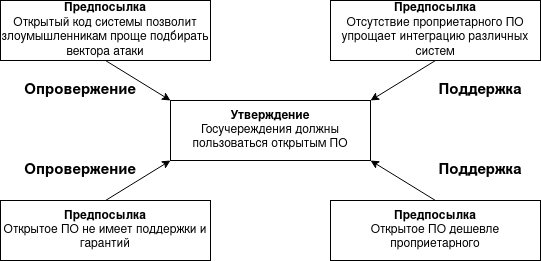
\includegraphics[scale=0.65]{Аргумент.png}}
 \caption{Пример аргументов, относящихся к применению открытого ПО.}
\end{figure}

%Помимо вышеуказанных структурных особенностей связи компонент аргументации могут дополнительно описываться следующими характеристиками:
%\begin{itemize}
%    \item Сила – мера того, насколько предпосылки соглашаются с утверждением, темой или опровергают их.
%    \item Общность – мера того, насколько утверждение или предпосылка раскрывает тему, а не ее конкретные примеры, иначе оно превращается в факт.
%    \item Авторитетность - характеристика того, насколько данное утверждение или предпосылка обоснована. Например высказывание ученого о глобальном потепленее авторитетнее высказывания политика.
%\end{itemize}

Аргументация присутствует почти во всех источниках информации: она встречается в бытовых спорах, дебатах, научном дискурсе. Особый вид политической аргументации – пропаганда является ключевым компонентом некоторых интернет-ресурсов.

За последнее десятилетие сильно вырос интерес к автоматическому выделению аргументации \cite{lippi2016argumentation}. Этому поспособствовал прорыв в области обработки естественного языка, заключающийся создании предобученных нейросетевых моделей с сильными обобщающими способностями \cite{mikolov2013efficient, devlin2018bert, radford2019language}. Несмотря на то, что данные модели содержат в себе знание общеизвестных и часто встречаемых фактов, выученных из больших коллекций \cite{petroni2019language}, они не способны применять узкоспециализированую информацию. Для решения данного недостатка используют графы знаний и другие онтологии \cite{sorokin2018modeling, chen2019multi}, однако их создание требует трудоемкий и долгий процесс ручной разметки данных экспертами. Автоматическое извлечение аргументации позволяет динамически извлекать специализированную информацию и структурировать ее.

В данной задаче отстутствует устоявшаяся постановка. В научной литературе существует несколько вариантов определения аргументации и соответстующих подходв к ее выделению. Из-за этого отсутствует общепринятый набор тестов и метрик, позволяющих оценить качество системы извлечения аргументации. Следствием отсутствия универсальной постановки задачи является небольшое число исследовательских групп, занимающихся аргументацией, наличие различных по постановке и небольших по размерам обучающих коллекций и почти полное отсутствие развития задачи на языках отличных от английского.

Проблему плохого покрытия языка можно решать созданием новых или параллельных \cite{fishcheva2019cross}  корпусов, а также методикой межязыкового переноса знаний \cite{ponti2020xcopa, eriguchi2018zero}. Данный подход заключается в обучении мультиязычной модели на одном языке для адаптации полученных знаний на других языкак.

В данной работе описывается исследование методов извлечения структуры и полемической позиции аргументации, а также способы адаптации данных методов для применения на русскоязычных корпусах с помощью подхода межязыкового переноса.

\subsection{Актуальность задачи}
Извлечение аргументации можно применить во многих прикладных сценариях:
\begin{itemize}
    \item Аргументация может быть задействована в экспертных системах для получения доводов "за"  и "против" относительно какого-либо утверждения.
    \item Аргументы можно использовать в голосовых помошниках и других системах, использующих базы знаний.
    \item Выделение аргументации применительно к научным текстам позволит лучше высторить структуру взаимосвязи между цитируемыми работами.
    \item Аргументация также может использоваться для оценки убедительности и логичности текстов.
    \item Аргументация может использоваться в нефактоидных вопросно-ответных системах для ответов на вопросы, требующие объяснений: "Почему было принято следующе решение?"
\end{itemize}

Один из самых показательных примеров применения аргументации является проект IBM Debater, который способен поддерживать сложный диалог с оппонентом для обоснования определенной точки зрения. В 2019 году система IBM Debater участвовала в споре с финалистом мирового чемпионата по дебатам Харишем Натараджаном, в котором на протяжении 15 минут смогла отстаивать свою точку зрения. Другим примером могут послужить голосовые помошники, получившие широкое распространение в последние годы. В лидирующих системах, таких как Siri, Алиса, Маруся, Alexa и Google Assistant для ответов на вопросы ищутся релевантные документы, которые потом цитируются в качестве ответа, однако они не способны агрегировать информацию из нескольких источников. Добавление аргументации поможет голосовым помошникам систематизировать информацию и обосновывать свои ответы. В качестве примера можно привести работу \cite{schiller2020aspect}, где по извлеченным примерам аргументации генерируется текст.

Из всего вышесказанного можно сделать вывод, что выделение аргументации с помощью методов глубокого обучения является перспективной и актуальной задачей. Научная ценность данной работы заключается в исследовании и систематизации текущих подходов к задаче извлечения аргументации, применении новых моделей и предоставлении замеров результатов их работы. Отдельной проблемой является и работа с множеством небольших, разнящихся в постановке задачи корпусов. Следствием является и проблема построения системы извлечения аргументации для русского языка. 

В работе приводится обзор и анализ существующих работ по извлечению аргументации, предлагаются новые подходы, основанные на переносе знаний (transfer learning), а также исследуется возможность межязыкового переноса знаний для получения модели, работающей на русском языке. Дополнительно проводится интерпретация работы модели: исследуется зависимость полученных результатов в зависимости от структурных особенностей компонент аргументации, таких как наличие отрицаний, сильно окрашенных слов или антонимии.

\section{Постановка задачи}
Целью данной работы является исследование существующих методов извлечения структуры и полемической позиции аргументации и разработка новых модельных подходов. 

Перед дальнейшими определениями необходимо пояснить термен "компоненты аргументации". Определение и набор компонент разнятся от работы к работе, но в общем случае можно выделить следующие сущности:

\begin{itemize}
    \item Фокус - центральный объект обсуждения.
    \item Тема - противоречивое утверждение относительно фокуса.
    \item Утверждение - фраза или предложение, поддерживающие или опровергающее тему.
    \item Предпосылка - фраза или предложение, поддерживающие или опровергающие или тему или предложение, основанное на фактах, а не на убеждении.
\end{itemize}

Под структурой аргумента подразумевается набор компонент аргументации и отношения связности или релевантности между ними. Например для темы "запрет ядерной энергии" утверждение "ядерная энергия вредна для окружающей среды" является релевантным, а утверждение "человеческий глаз воспринимает около миллиона оттенков" релевантным не является. Отношение релевантности является бинарным отношением между компонентами аргументации.

Задача определения полемической позиции заключается в определении типа связи между релевантными компонентами аргументации. Релевантное теме утверждение может как соглашаться с темой, так и ее опровергать. Задача классификации связей между релевантными компонентами аргументации в два класса поддержки и атаки называется определением полемической позиции. Как видно из определения, полемическая позиция применима исключительно к релевантным компонентам аргументации и представляет собой два взаимоисключающих класса связей.

Для достижения поставленной в работе цели необходимо решить следующие подзадачи:

\begin{enumerate}
	\item Произвести обзор существующих решений и корпусов, выделить наиболее подходящие постановки.
    \item Воспроизвести избранные работы или получить новые базовые решения.
    \item Предложить или адаптировать новые модельные подходы для извлечения аргументации.
    \item Провести анализ полученной модели с целью интерпретации полученных результатов.
\end{enumerate}

\section{Обзор подходов к извлечению аргументации}

\subsection{Обзор корпусов}
Задача извлечения аргументации решается в различных постановках. Общей идей является выделение компонент аргументации и определение связей между ними. Наиболее серьезные работы с применением машинного обучения, посвященные теме извлечения аргументации, датируются 2014 годом. В работах \cite{aharoni2014benchmark, rinott2015show} предлагается корпус аргументации на 2500 примеров. В качестве компонент аргументации рассматриваются три сущности:
\begin{itemize}
    \item Тема - короткая противоречивая фраза, определяющая центральный объект обсуждения (фокус).
    \item Контекстно-зависимое утверждение - краткая фраза, напрямую подтверждающая или опровергающая тему.
    \item Контекстно-зависимая предпосылка - участок текста, напрямую поддерживающий контекстно-зависимое утверждение в рамках данной темы.
\end{itemize}

Задача поставлена следующим образом - по заданной теме и коллекции текстов из википедии необходимо выделить контекстно-зависимые утверждения и предпосылки. Этап выделения компонент аргументации разделен на две подзадачи. Сначала предлагается выделить предложения, содержащие компоненты аргументации, после чего выделить непрервыне участки текста (фразы), которые являются непосредственно предпосылкой или утверждением. Таким образом решается задача выделения структуры аргументации. Как следует из определений, в данном корпусе отсутствует связь противоречия (атаки, противопоставления) между компонентами, поэтому отсутствует возможность выучить полемическую позицию аргумента. Стоит отметить, что задача выделения непрервыного участка текста в качестве компонент аргументации требует сложной разметки, из-за чего в следующих работах отказываются от этого этапа и решают задачу извлечения компонент на уровне предложений.

Дополнительно поставлена задача классификации предпосылок в три класса - прецедентные (Anecdotal), т.е. основанные на каком-либо случае; экспернтые (Expert), т.е. высказывание авторитетного источника; исследовательские (Study), т.е. результаты какого-либо научного исследования.



В работе \cite{shnarch2018will} предлагается новый корпус IBM Evidence Search размером 5700 примеров извлечения контекстно-зависимых предпосылок по темам. В данном корпусе происходит изменение постановки задачи. В предыдущих работах предпосылки имели связь с утверждениями, которые в свою очередь имели связь с темами, теперь предпосылки связаны напрямую с темами. В данном корпусе решается задача определения релевантности предпосылки по отношению к теме, т.е. решается задача извлечения структуры аргументации. В разметке отсутствует полемическая позиция предпосылки - поддержка или опровержение темы.

Предлагается два корпуса - SLD (strong labeled data, т.е. данные полученные с помощью человеческой экспертизы), а так же WLD (weak labeled data, т.е. данные, полученные автоматическими правилами), однако корпус WLD не предоставлен. В работе исследуется зависимость качества модели определения релевантности между предпосылкой и темой в зависимости от соотношения корпусов WLD и SLD. Показано, что использование данных, полученных автоматически повышает итоговое качество модели на несколько пунктов с 70\% до 72-74\% точности классификации, усредненной по темам.

В работе \cite{stab2018cross} предлагается корпус UKP Sentential Argument Mining Corpus. Рассматриваются пары сущностей "тема" и "утверждение", определяется наличие связи и ее тип. В отличие от предыдущих работ, тема не является противоречывым высказыванием, а вместо этого представляет собой центральный объект обсуждения (фокус). Утверждение является предложением, которое может как поддерживать или опровергать фокус, так и не иметь к нему отношения, что позволяет решать и задачу определения структуры аргументации и полемической позиции. Примеры: тема - "ядерная энергия", поддерживающее утверждение - "ядерная энергия уменьшает парниковый эффект". В корпусе представлено 25000 пар тем и утверждений по 8 темам. 

В работе исследуется способность моделей работать на новых темах, т.е. обобщать свои знания на домены, которые раньше не были выучены моделью. Несмотря на ограниченный набор тем, данный корпус одним из первых позволяет решать одновременно и задачу извлечения структуры аргументации и определения полемической позиции. Корпус отсутствует в открытом доступе.

В работе \cite{levy2018towards} подробнее описываются техники автоматического получения корпусов на примере задачи определения релевантности утверждения по отношению к теме. В качестве основного способа предлагается использовать правила, основанные на определенных лексических маркерах. Например предполагается, что часто встречаются шаблоны вида \textbf{<someone>argued that<claim>}. В корпусе отсутствует полемическая позиция и решается только задача определения структуры аргументации. В качестве замеров эффективности обученная на подобном корпусе модель замеряется на UKP Sentential Argument Mining Corpus и получает результаты сравнимые с моделями, предложенными в оригинальной работе.

Исследование \cite{bar2017stance} полностью посвещено задаче определения полемической позиции утверждений по отношению к теме. В корпусе IBM Claim Stance предоставлено 2400 пар тем и утверждений связанных отношением поддержки или атаки. Отсутствуют примеры утверждений не связанных с темами, поэтому отсутствует возможность извлечь структуру аргументации.


Отдельно стоит отметить и задачу определения качества аргументации, которой посвещен целый ряд работ \cite{gretz2020large, toledo2019automatic, gleize2019you}. В данной задаче необходимо определить качество утверждения по отношению к теме. Решение данной задачи позволяет отсортировать утверждения, чтобы использовать наиболее подходящие в целевой задаче. Сущестует несколько постановок данной задачи: присваивание утверждению некоторой величины от 0 до 1, отражающей его качество, или попарное сравнение двух утверждений с выбором наилучшего. 

В данных работах рассматриваются поддерживающие утверждения релевантные теме, поэтому невозможно обучить модель на этих корпусах ни определению полемической позиции, ни структуре аргументации, однако нельзя не отметить полезность подобного ранжирования в полномасштабной системе извлечения аргументации.

В работе \cite{toledo2020multilingual} предлагается два мультиязычных корпуса для извлечения аргументации. В первом корпусе ArgsEN было предоставлено 30000 пар тем и утверждений, у которых размечена полемическая позиция и качество аргумента. Помимо этого предоставлен корпус EviEN, состоящий из 35000 пар предпосылок, в котором размечена и полемическая позиция и релевантность.

Свой подход к аргументации развивается и в исследовательской команде Webis. В корпусе Webis Debate 16 \cite{webis16} предлагается классифицировать предложения в два класса - нейтральные и содержащие утверждение. В данной текстовой коллекции утверждения не привязаны к теме или любой другой компоненте аргументации; данная постановка не позволяет выделить ни структуру аргументации, ни полемическую позицию внутри нее.

Нельзя не внести в обзор и такую задачу как логический вывод (Textual Entailment, Natural Languge Inference). Данная задача напрямую не занимается извлечением аргументации, но задачи имеют схожую постановку: требуется по тексту и гипотезе понять отношение между ними. Видов отношений 3: нейтральное отношение, поддержка, противоречие. Примеры:
\begin{verbatim}
Текст: A man inspects the uniform of a figure in some East Asian country.
Гипотеза: The man is sleeping
Отношение: Contradiction

Текст: An older and younger man smilin
Гипотеза: Two men are smiling and laughing at the cats playing on the floor
Отношение: Neutral

Текст: A black race car starts up in front of a crowd of people
Гипотеза: A man is driving down a lonely road.
Отношение: Contradiction
\end{verbatim}

Задача NLI интересна тем, что как и в задачах извлечения аргументации присутствует несколько компонент (текст и гипотеза), между которыми необходимо найти связь. Вместо оригинальной постановки, в которй требовалось классифицировать отношение между двумя предложениями в 3 класса, можно факторизовать задачу в две подзадачи: определить релевантна ли гипотеза тексту, после чего определить при условии релевантности поддерживает ли или опровергается текст гипотезой. Данная формулировка очень похожа на этапы извлечения аргументации, а именно на извлечение структуры и последующее определение полемической позиции.

Существует несколько корпусов для решения подобной задачи: Stanford NLI \cite{snli:emnlp2015}, Multi-Genre NLI, TERRa. В отличие от корпусов аргументации, размер корпусов логического вывода измеряется не в тысячах примеров, а в сотнях тысяч. Более того, корпуса для этой задачи встречаются на нескольких языках, в том числе и русском.

Как было сказано в определении предпосылки, важно, чтобы предпосылка не являлась убеждением или верованием, а имела под собой веские основания. Во всех описанных выше корпусах, где предлагалось работать с предпосылками, предполагалось, что эта закономерность заложена в данные. В соревновании \textbf{CheckThat!} \cite{barron2020overview} при конференции CLEF с 2020 задача верификации предпосылок решается целенаправленно. В данном соревновании представлены следующие дорожки, собранные из данных социальной сети Twitter:
\begin{itemize}
    \item \textbf{Значимость (Check Worthiness)} - даны сообщения пользователей, необходимо отранжировать их по значимости, т.е. таким образом, чтобы на первых местах оказались те сообщения, которые необходимо верифицировать в первую очередь.
    \item \textbf{Выделение предпосылок (Claim Retrieval)} - дано утверждение, представляющее из себя некое сообщение из твиттера, и набор уже верифицированных утверждений. Необходимо отранжировать верифицированные утверждения, чтобы понять, можно ли с их помощью подтвердить целевое утверждение. Данный трек доступен только на арабском языке.
\end{itemize}

Похожим образом построен и корпус FEVER (Fact Extraction and VERification) \cite{thorne2018fever}. Необходимо по набору утверждений и статей из википедии найти участки текста, подтверждающие целевое утверждение.

В работе \cite{abbott2016internet} предоставляется Internet Argument Corpus v2. В данной коллекции размечены пары сообщений из интернет-форумов. Сообщения разбиты на пары-вопрос-ответ и размечены по следующим критериям:
\begin{enumerate}
    \item Согласие или несогласие - число от -5 до 5, отражающее полемическую позицию ответа к вопросу.
    \item Эмоциональность или факты - число от -5 до 5, отражающее насколько в ответе используются факты, а не эмоции и убеждения отвечающего.
    \item Сарказм - число от 0 до 1, отражающее число разметчиков, посчитавших ответ саркастичным, а не серьезным.
\end{enumerate}
Как видно из описания данный корпус предоставляет определенную разметку веб-дискурса, из которой можно определенными эвристиками получить корпус для извлечения структуры и полемической позиции аргументации.

В более ранних работах встречались небольшие корпуса из очень узких тематических областей. В работах \cite{palau2009argumentation, ronzano2015dr} предоставлена схожая разметка в юридических документах и научных статьях соответственно. Разметка представляет с собой связи между предложениями внутри текстов - как предложения поддерживают друг друга, чтобы итоговый текст был связным и убедительным. 

Дополнительно стоит отметить и примеры политической аргументации, содержащиеся в корпусе трека SemEval 2020 Task 11 Propaganda detection in news articles \cite{da2020semeval}. В данном соревновании предлагается выделить участки новостных статей, содержащих аргументацию, а также классифицировать их в такие приемы, как ложная аналогия, подмена тезиса, эксплуатация двусмысленных выражений, сведение аргументации к универсально осуждаемой теме и другим приемам убеждения оппонента. Пропаганду также можно свести и к примерам "ложной" аргументации, так как она скорее нацелена убеждение читающего, а не на установление истины.

\subsection{Обзор существующих решений}

Было создано несколько систем для извлечения аргументации, работающих с различными постановками задачи.

Первая  рассматриваемая система MARGOT \cite{lippi2016margot} придерживается определений контекстно-зависимых утверждений и предпосылок из работы \cite{aharoni2014benchmark}. По заданной теме к тексту последовательно применяется несколько моделей - модель определения предложений, содержащих компоненты аргументации, и модель выделения компоненты внутри предложения, после чего компоненты аргументации связываются отношением поддержки. Предложенные модели основаны на методах машинного обучения над признаками, выделенными из синтаксиса предложений.

Система MARGOT решает задачу извлечения аргументации в одной из самых ранних постановок, от которой отказались в последующих работах. В данной постановке отсутствует отношение противоречия, что не позволяет полностью определить ни структуру, ни полемическую позицию аргументации. Более того в данной постановке дополнительно происходит выделение компонент аргументации внутри предложений, как коротких непрерывных участков фраз. От данной подзадачи впоследствии отказались в пользу решения задачи на уровне предложений.

Targer \cite{chernodub2019targer} - система направленная на анализ текстов с целью изучения их аргументационной структуры. В системе предлагается использовать подход классификации последовательностей слов (Sequence Tagging), подобный задаче распознавания именованных сущнностей, для разбиения текста на фразы и выделения связей между ними. Данная система работает в рамках определенного текста и не способна связывать произвольные компоненты аргументации, выделенные из различных источников.


ArgumentText \cite{daxenberger2020argumentext} - данная система отличается от предыдущих постановкой задачи. Вместо поиска участков текста, которые являются компонентами аргументации и выделения отношений между ними, производится поиск предложений, напрямую поддерживающих или опровергающих тему. ArgumenText представляет собой многоступенчатую систему извлечения аргументации, в рамках которой решается и задача кластеризации утверждений по теме, поиск и классификация релевантных документов.


\subsection{Вывод}
Как видно из обзора работ существует множество подходов к задаче извлечения аргументации, как и существует несколько постановок. Также есть и ряд подзадач, таких как верификация и ранжирование утверждений по качеству или определение противоричивости темы.

Основными критериями для выбора корпусов служили следующие критерии:

\begin{itemize}
    \item Возможность напрямую решать или задачу определения структуры или определения полемической позиции аргументации. В то время как сущетсвует множество различных постановок задачи извлечения аргументации, а так же вспомогательных задач, в рамках данной работы было решено сфокусироваться на основных задачах извлечения аргументации.
    \item Возможность сравнить свое модельное решение с заявленными метриками качества. Некоторые работы или не имеют заявленных чисел или имеют невоспроизводимые результаты (замеры качества с помощью экспертов), или используют в обучении дополнительные закрытые наборы данных, которые не позволяют адекватно сравнить полученные системы.
\end{itemize}

По этим причинам были выбраны следующие корпуса:
\begin{enumerate}
    \item Новостной корпус пропаганды из соревнования SemEval \cite{da2020semeval}.
    \item Корпус для построения структуры аргументации IBM Evidence Search из работы  \cite{shnarch2018will}
    \item Корпус для определения полемической позиции ArgsEN и корпус для одновременного определения полемической позиции и структуры аргументации EviEN из работы \cite{toledo2020multilingual}.
    \item Корпус из задачи логического вывода SNLI \cite{snli:emnlp2015} для исследования применимости закономерностей, выученных на задаче логического вывода в задаче извлечения аргументации.
    \item Корпус задачи логического вывода TERRA на русском языке
\end{enumerate}



\section{Методы решения задачи}

В рамках проблемы извлечения аргументации необходимо решить две подзадачи: выделение структуры аргумента и определение полемической позиции. Обе эти задачи являются задачами классификации. Формально даны два текста (предложения) $A = (a_1, a_2, ..., a_n)$ и $B = (b_1, b_2, ..., b_m)$, где $a_i, b_j$ - слова. Необходимо для пары компонент аргументации $A,B$ определить класс отношения $Y = (y_1, ..., y_k)$, т.е. смоделировать функцию ($P$ обозначает вероятность):

\begin{equation*}
    f(A, B, y_i) = P(y_i| A, B)
\end{equation*}

В задаче определения структуры аргументации присутствует два класса: отношение релевантности и нерелевантности (нейтральное). В задаче определения полемической позиции также два одношения: поддержка и опровержение (атака).

В задаче определения пропаганды присутствует 14 классов пропаганды, постановка задачи остается похожей: дан новостной текст $X = (x1, ..., x_n)$, дан участок $x_i, ..., x_i + k$, необходимо классифицировать данный сегмент в один из классов $Y = (y_1, ..., y_14)$:
\begin{itemize}
    \item Сильно окрашенная лексика. Пример: ".. a lone lawmaker’s childish shouting."
    \item Навешивание ярлыков и имен. Пример: "Republican congressweasels"
    \item Повторение. Заключается в повторении тезиса для закреплении концепции в голове у слушателей.
    \item Преувеличение или приуменьшение. Пример: "Democrats bolted as soon as Trump’s speech ended in an apparent effort to signal they can’t even stomach being in the same room as the president"
    \item Сомнения. Пример: "Is he ready to be the Mayor?"
    \item Взывание к страхам и предрассудкам. Пример: "stop those refugees; they are terrorists"
    \item Сбор под флагом, т.е. взывание к аудитории на почве общей какой-либо общей идентичности (национальности, пола и т.п.). Пример: "entering this war will make us have a better future in our country"
    \item Упрощение причины, т.е. упор на какую-либо первопричину в проблеме с множеством факторов. Пример: "If France had not declared war on Germany, World War II would have never happened."
    \item Слоганы - любые яркие фразы, взывающие к эмоциям. Пример: "Make America great again!"
    \item Диктатура - представление ограниченного выбора в задаче, где существует большее число вариантов решение проблемы. Пример: "There is no alternative to war."
    \item Терминирующие размышления клише - фразы дискредитирующие критичекское размышление по теме обсуждения. Пример: "никто не идеален" или "нельзя изменить человеческую натуру"
    \item Whataboutism - перевод темы для занятия более высокой моральной позиции. Пример: "А у вас права ущемляют!".
    \item Сведение вопроса к заведомо осуждаемой теме. Пример: "Only one kind of person can think this way: a communist!"
    \item Красная сельдь - представление нерелевантной информации для отвращения внимания. 
    \item Стадность - захват мнения через представление позиции, как поддерживаемой большинством. Пример: "Would you vote for Clinton as president? 57\% say yes."
    \item Нарочитая расплывчатость и неясность.
    \item Соломенный человек - подстановка похожего утверждения вместо утверждения оппонента с его последующим опровержением.
\end{itemize}

В задаче извлечения пропаганды дополнительно стоит задача нахождения участков текста, являющихся пропагандой, т.е. для текста $X = (x_1, ..., x_n)$ определить бинарный набор меток $Y = (y_1, ..., y_n)$, где $y_i = 1$, если слово $x_i$ входит в сегмент с пропагандой, иначе $y_i = 0$. Для решения проблемы необходимо построить модель:

\begin{equation*}
    f(X, Y) = P((y_1, y_2, ..., y_n) | (x_1, x_2, ..., x_n))
\end{equation*}

\subsection{Современные подходы к обработке естественного языка}
За последнее десятилетие область обработки текстов значительным образом преобразилась. Тексты хуже поддаются обработке различными нейросетевыми алгоритмами из-за их дискретной структуры. Ранние работы, основаные на классических метотдах машинного обучения используют методики Bag of words или Tf-Idf для векторизации текста. Данные подходы не способны улавливать сложные закономерности, так как не учитывают порядок и внутреннюю структуру текста, поэтому их зачастую дополняют информацией о синтаксической структуре предложения и другуми экспертными признаками.

В 2013 году с появлением word2vec \cite{mikolov2013efficient} началось стремительное развитие применения нейросетей в обработке текстов. Основная идея данного подхода заключается в выучивании векторов слов для моделирования дистрибутивной гипотезы: слова, встречающиеся в схожих контекстах, имеют близкие значения.

Долгое время стандартом моделей была одна из векторизаций (word2vec, glove, fasttext) дополненная рекуррентной нейросетью (LSTM, GRU) \cite{hochreiter1997lstm} и финальным слоем специфичным для задачи.  В данном подходе рекуррентные нейросети выучивыают контекстные закономерности в рамках определенной задачи.

Со временем начали появляться модели общего назначения для задачи восприятия естественного языка (Natural Language Understanding). Данные модели не требуется обучать с нуля, вместо этого они проходят длительное предобучения на общей задаче моделирования языка \cite{Peters:2018}: для последовательности $X = (x_1, x_2, .., x_k)$ слов из словаря $V = (v_1, v_2, ..., v_n)$ моделируется следующая закономерность:

\begin{equation*}
    f(X, v_i) = P(x_{k+1} = v_i| (x_1, ..., x_k))
\end{equation*}

В настоящий момент большие предобученные модели основанные на архитектуре трансформер являются доминирующими почти во всех областях обработки текстов. Особенностью данной архитектуры является полный отказ от рекуррентности в пользу механизма внимания.

Механизм внимания пришел из задачи машинного перевода, где главным подходом была архитектура Seq2Seq \cite{sutskever2014sequence}. Данная архитектура состоит из энкодера, сжимающего предложение в вектор, и декодера, разжимающего данный вектор в текст на другом языке. Одна из главных заявленнных проблем - данный подход плохо работает на длинных предложениях. Это связано с тем, что при сжатии в вектор фиксированного размера теряется очень большой объем информации.

Прорыв произошел с разработкой механизма внимания \cite{bahdanau2014neural}. Данный механизм позволяет сопоставлять вектор предложения в декодере с соответствующими состояними в энкодере. Каждому состоянию энкодера, соответствуещему определенному токену, на каждом шаге при декодировке ставится в соответствие вес, после чего состояния энкодера усредняются с данными весами и используются для расширения внутреннего состояния декодера.

Архитектура трансформер \cite{vaswani2017attention} основывается на механизме внимания. В рамках нейросетевой модели механизм внимания применяется от каждого слова предложения ко всем словам предложения. С последовательным применением нелинейности данный механизм применяется несколько раз на каждом слое нейросети, после чего на выходе получается векторное представление для каждого слова в предложении, насыщенное контекстуальной информацией.

Одной из самых популярных предобученных архитектур является BERT \cite{devlin2018bert}. Данная модель обучалась на коллекции Book Corpus задаче маскированного языкового моделирования и предсказания следующего предложения. Задача маскированного языкового  моделирования заключается в предсказании одного и более слов в предложении. Таким образом после обучения модель имеет внутри себя знания о структуре языка, о мире, поэтому ее легко адаптировать для различных вариаций задачи понимания естественного языка.

Это подтверждается успехом подобных моделей почти во всех современных задачах естественного языка и особом соревновании GLUE Benchmark. Данное соревнование содержит в себе ряд задач на понимание языка, которые при небольшом дообучении решаются моделями подобными BERT на уровне человека или выше.

В рамках данной работы было выбрано использовать нейросетевые подходы на основе предобученных моделей-трансформеров, так как данные модели показывают наилучшие результаты на большинтстве задач обработки естественного языка.

\subsection{Модели для извлечения аргументации}
Для извлечения аргументации необходимо решить подзадачи построения структуры и определения полемической позиции аргументации. В рамках рассмотренных корпусов компонентами аргументации являются темы и утверждения или предпосылки. Стоит дополнительно отметить, что не у всех представленных текстовых коллекций присутствуют какие-либо базовые решения и замеры качеств.

В работе, сопровождающей корпус IBM Claim Stance \cite{bar2017stance} предложенная модель представляет собой метод опорных векторов (Support Vector Machine) над векторизацией мешка слов (Bag of words). 

В работе \cite{toledo2020multilingual} для определения полемической позиции, структуры и качества аргумента предлагается система, основанная на предобученной модели $BERT$, однако сама архитектура не раскрывается.

Отсутствие предложенных базовых решений приводит к необходимости использования заимствованных или альтернативных подходов. Для классификации отношений между двумя парами компонент аргументации предлагается модель $BERT_{basic}$. В рамках данной модели входы, представляющие из себя две компоненты аргументации объединяются в один текст, разделенные специальным символом \textbf{[SEP]}. После этого входная последовательность проходит сквозь слои модели, в результате чего механизм внимания, интерпретируя закономерности между двумя текстами, выдает сжатый вектор. Далее данный вектор подается в линейный слой, который решает задачу классификации.

Данная модель вдохновлена оригинальной методикой предобучения модели $BERT$, в которой аналогичным образом решалась задача предсказания следующего предложения (Next sentence prediction) - необходимо было определить, является ли одно предложение продолжением другого. 

Стоит отметить, что сложность работы модели квадратична относительно длины входной последовательности, и, возможно, данный подход не был бы эффективен в сценарии, где необходимо было бы быстро извлечь аргументацию из большого количества текстов. Альтернативой первой модели служит модель $BERT_{vectorized}$, в которой предлагается независимо пропустить две компоненты аргументации через слои предобученной модели, после чего сконкатенировать их векторные представления и передать для классификации в линейный слой. За счет уменьшения длины входных данных уменьшается и время работы модели, однако компоненты аргументации векторизуются без информации друг о друге, что может привести к потере качества.

В работе \cite{sun2020self} предлагается подход улучшения качества модели за счет добавления интерпретируемости. Данная модель $BERT_{SE}$ представляет собой дополненую модель $BERT_{basic}$: в конце после прохождения всех слоев трансформера для каждого слова на выходе имеется вектор, отображающий контекстуальную информацию предложения внутри текста, т.е. каждая входная последовательность $X = (x_1, ..., x_n)$ отображается в последовательность векторов $H = (h_1, ..., h_n), h_i = (h_{i_1}, ..., h_{i_k}$, где $k$ - размерность модели.
В обычной задаче классификации берется выход на первом слове $h_1$, т.е. на спецсимволе начала предложения \textbf{[CLS]}. В модели $BERT_{SE}$ предлагается взять всевозможные участки текста вида $span(i, j), i \leq j, |span(i, j)| = k$ и с помощью линейного слоя проставить каждому участку текста некое число $s_q$, отражающее важность данного участка текста в финальной классификации. После этого $s_q$ превращается в множители для взвешенной суммы участков текста, финальное векторное представление $t$ для классификации считается следующим образом:

\begin{equation*}
    \alpha_i = \frac{\exp(s_i)}{\sum_{j=1}^{k}\exp(s_j)} \\
\end{equation*}
\begin{equation*}
        t=\sum_{q=1, i \leq j}^{k} \alpha_q * span(i, j)
\end{equation*}
Далее взвешенное представление всех участков $t$ подается в линейный слой для решения задачи классификации. Множители $\alpha_i$ могут использоваться для интерпретации модели, так как они отображают самый важный для классификации непрерывный участок текста.


Дополнительн для исследования применимости знаний, полученных на корпусе SNLI предлагается обучить модель $BERT_{basic}$ на задаче логического вывода и исследовать следующие сценарии: применимость модели без дообучения на корпусах извлечения аргументации (Zero Shot) и исследование предобучения модели на корпусе SNLI для дообучения целевой задаче извлечения аргументации. 

\subsection{Модели для обнаружения пропаганды}
Задача извлечения пропаганды является новой задачей, к которой не было применено никаких существующих подходов. В дорожке по детекции, где было необходимо выделить участки текста, являющиеся пропагадной, было предложено начать с базовых моделей из работы \cite{lample2016neural}. Первая модель $LSTM$ основывается на одноименной архитектуре рекуррентных нейросетей. На вход модели подается текст, представляемый последовательностью слов $X = (x_1, .., x_n)$, после чего данный текст проходит через LSTM-слои и преобразуется в контекстные вектора $H = (h_1, ..., h_n), h_i = (h_{i_1}, ..., h_{i_k}$. Каждому слову на основе полученных векторов независимо ставится метка 0 (отсутствие пропаганды) или 1 (пропаганда) с помощью применения линейного слоя. Данные метки составляют список меток $Y = (y_1, ..., y_n)$, который однозначно определяет все участки пропаганды в тексте.

Модификацией данной модели является $LSTM_{CRF}$. Предлагается устранить недостатки предудыщей модели за счет замены финального слоя на слой Conditional Random Field (CRF). Данный слой выучивает возможные переходы и моделирует всю последовательнсть $Y$ одновременно.

В качестве более сложных моделей предлагается использовать предобученную модель $BERT$ для векторизации входной последовательности и аналогично с предыдущими моделями в качестве выходных слоев испытать и линейный слой и CRF.

Также было решено позаимствовать архитектуру $LaserTagger$ из работы \cite{malmi2019encode}, так как данная модель зарекомендовала себя для классификации длинных последовательностей. Основная идея модели заключается в том, чтобы аналогично задаче машинного перевода, используя архитектуру "encoder-decoder" поставить каждому слову соответствующую метку.

Для улучшения работы модели $LaserTagger$ было предложено два дополнительных механизма Label Smoothing и Teacher Forcing. Техника label smoothing заключается в преобразовании меток класса из 0 и в более "мягкие", такие как 0.2 и 0.8. Данная методика позволяет сгладить резкие изменения градиентов на ошибках модели. Teacher forcing заключается в подаче авторегрессионной модели не только правильрных меток, но и предсказанных ею неверных меток. Таким образом модель становится более устойчивой к ошибкам и исследуюет во время обучение больше различных сценариев. 

\begin{figure}[h!]
\centering
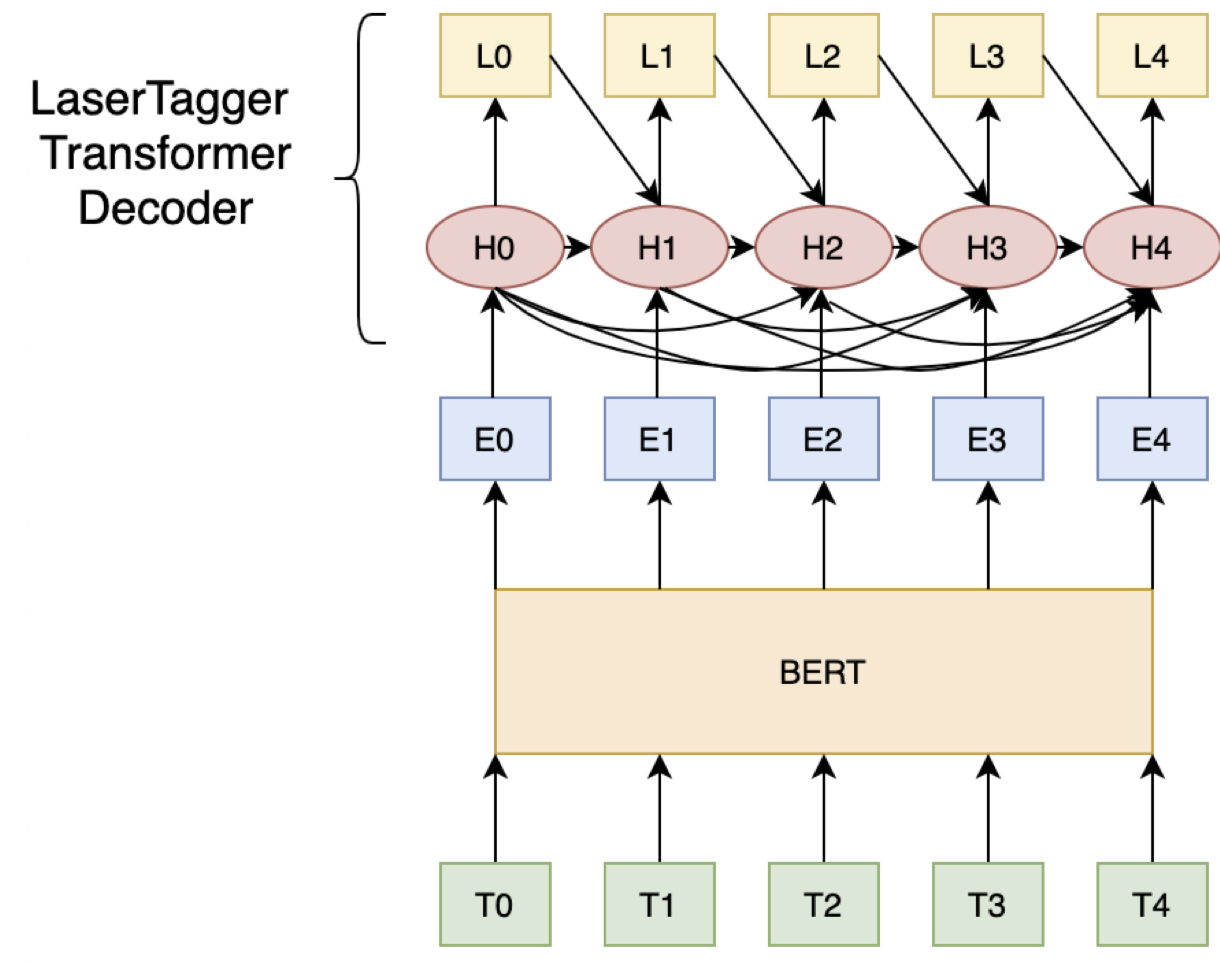
\includegraphics[scale=.5]{lasertagger.png}
\caption{Архитектура LaserTagger.}
\label{Problem_Picture}
\end{figure}


Во второй дорожке требовалось для каждого сегмента пропаганды определить, к каким классам он относится. Задача поставлена на уровне предложений, однако решать ее как классификацию предложений невозможно: в одном предложении может содержаться более одного участка пропаганды. Для этого было решено адаптировать модельный подход $RBERT$ \cite{wu2019enriching}, заключающийся в обрамлении нужных участков текста спецсимволами. Таким образом модели выделяется нужная фраза, что позволяет при необходимости работать с разными участками текста в рамках одного предложения.

\begin{figure}[h!]
\centering
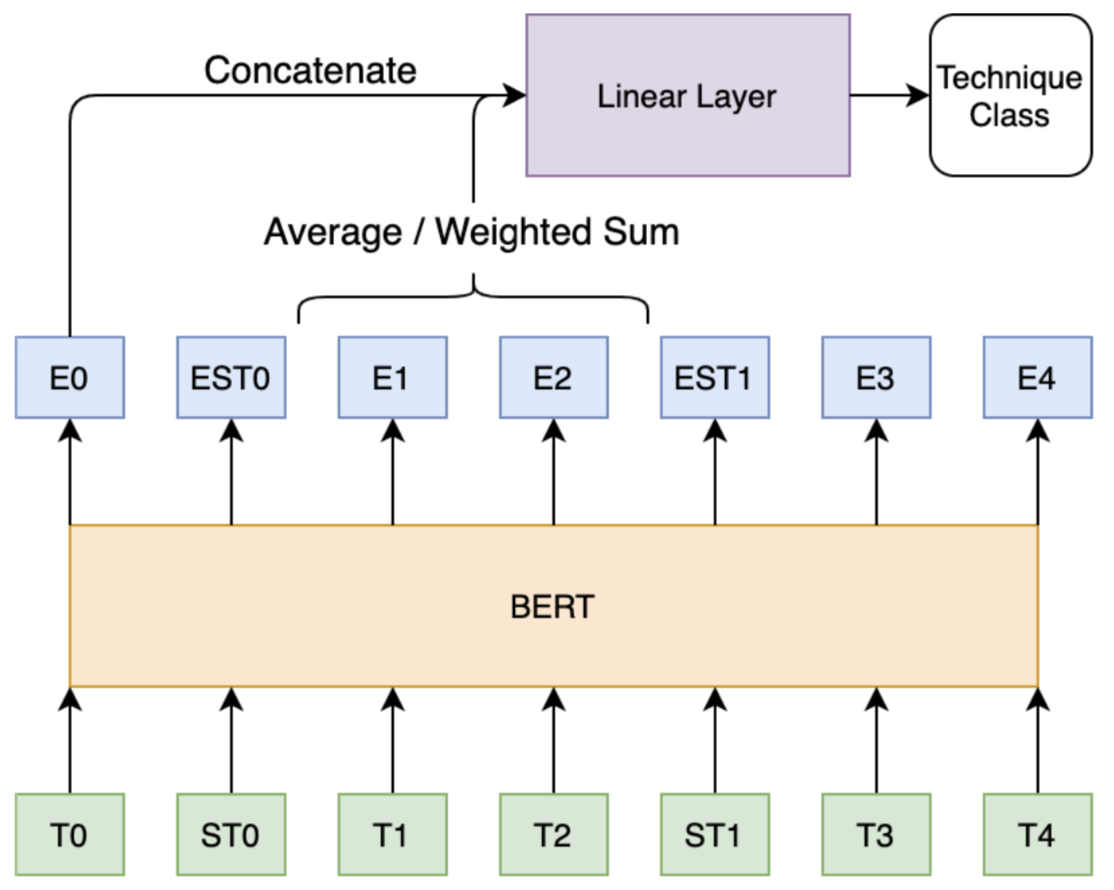
\includegraphics[scale=.5]{rbert.png}
\caption{архитектура R-BERT.}
\label{Problem_Picture}
\end{figure}


\subsection{Методы для межязыкового переноса знаний}

В области обработки естественного языка наиболее распространены англоязычные корпуса. Английский язык получает наибольшее покрытие задачами, однако проверка работоспособности моделей на других языках из-за этого остается плохо исследованной проблемой.

Методов получить модель для другого языка несколько, направления межязыкового переноса активно развивается в настоящее время. Самым простоым способом является создание параллельного корпуса. Использование профессиональных переводчиков затратно и треюует много времени, поэтому достаточно часто для первичной проверки гипотез прибегают к автоматизированным средствам перевода.

Второй подход заключается в адаптации мультиязычной модели, т.е. модели предобученной на корпусе из различных языков. Считается, что для представлений одних и тех же слов на разных языках модель имеет схожие векторные представления, которые "замораживаются", т.е. не обучаются дальше. После этого данная модель дообучается на конкретной задаче на тех языках, на которых данная задача доступна, а качество замеряется уже на целевом языке.


\subsection{Выводы}

В результате обзора современных нейросетевых подходов были выбраные следующие модели для задачи извлечения аргументации:
\begin{itemize}
    \item Модель $BERT_{basic}$, т.к. она является базовой вариацией модели классификации, основанной на больших предобученных моделях.
    \item Модель $BERT_{vectorized}$ для исследования важности применения механизма внимания между компонентами аргументации.
    \item Модель $BERT_{SE}$ для исследования интерпретируемости результатов.
\end{itemize}

Для извлечения пропаганды были предложены две модели:
\begin{itemize}
    \item Модель, основанная на рекуррентной нейросети $LSTM$, так как это хорошее базовое решение, зарекомендовавшее себя в задачах классификации последовательностей.
    \item Модель $LaserTagger$, так как она зарекомендовала себя на задачах классификации длинных последовательностей.
    \item Модель $RBERT$ для классификации участков текста, так как она позволяет выделить интересующий участок пропаганды.
\end{itemize}

Для исследования переноса знаний на русский язык было выбрано перевести корпус IBM Claim Stance с помощью автоматизированного сервиса Google Translate и применить подход с заморозкой входных слоев мультиязычной модели $BERT_{multilingual}$ для дальнейшего замера качества на переведенном корпусе.
\section{Програмная реализация}
В качестве языка для реализации работы\footnote{https://github.com/hawkeoni/Thesis} был выбран Python 3.6. Данный язык позволяет быстро разрабатывать простые сервисы и имеет ряд библиотек для работы с нейросетевыми моделями. В качестве фреймворка для глубокого обучения используется Pytorch 1.6.0 и библиотека AlenNLP 1.1.0.

Кодовую базу можно разделить на несколько модулей:

\begin{itemize}
    \item Модуль обработки корпусов (800 строк) - данный код отвечает за обработку текстовых коллекций в форматы для обучения. Исходные форматы корпусов в форматах CSV, JSON, XML, MySQL dump были преобразованы в человекочитаемый формат JSONL.
    \item Модуль моделей (500 строк). В данном модуле написаны нейросетевые архитекутры и классы для взаимодействия с ними.
    \item Модуль обучения (500 строк). В данном модуле написаны циклы обучения, подсчет метрик, интеграции с системой отслеживания экспериментов\footnote{https://wandb.ai/hawkeoni}.
    \item Веб-сервис (250 строк) - реализован стенд для удобного взаимодействия с моделями на микрофреймворке Flask 1.1.1.
\end{itemize}

Выбор библиотек Pytorch и AllenNLP обоснован их простотой и возможностью быстрого прототипирования нейросетевых архитектур. Выбор микрофреймворка Flask для веб-сервиса был сделан из-за возможности легко создать веб-приложение на несколько страниц для взаимодействия с моделями.

Обучение происходило удаленно на сервере DataCrunch\footnote{https://datacrunch.io/} с видеокартами Tesla V100 с 16Гб видеопамяти. Процесс обучения в зависимости от корпуса занимал от 30 минут до 8 часов.

\begin{figure}[h!]
\centering
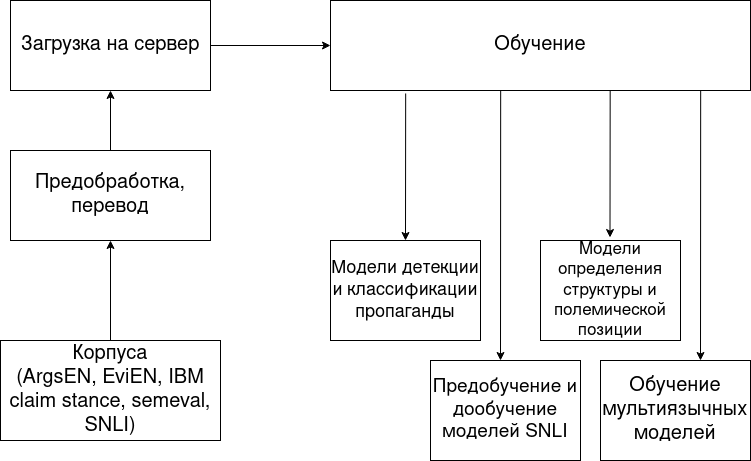
\includegraphics[scale=.5]{Комплекс.png}
\caption{Процесс обучения модели.}
\label{Problem_Picture}
\end{figure}


Для исследования эффективности работы моделей извлечения аргументации было создано веб-приложение. Веб-приложение содержит в себе одну страницу для взаимодействия с моделями. На странице предоставлены поля для компонент аргументации и выбора моделей. После заполнения полей и выбора моделей на странице с помощью языка JavaScript отображается результаты работы моделей определения структуры аргументации (релевантности) и полемической позиции (поддержка или атака).

\begin{figure}[H]
 \captionsetup{justification=raggedright,singlelinecheck=false,labelfont=bf,labelsep=period,name={Рисунок}}
 \centering{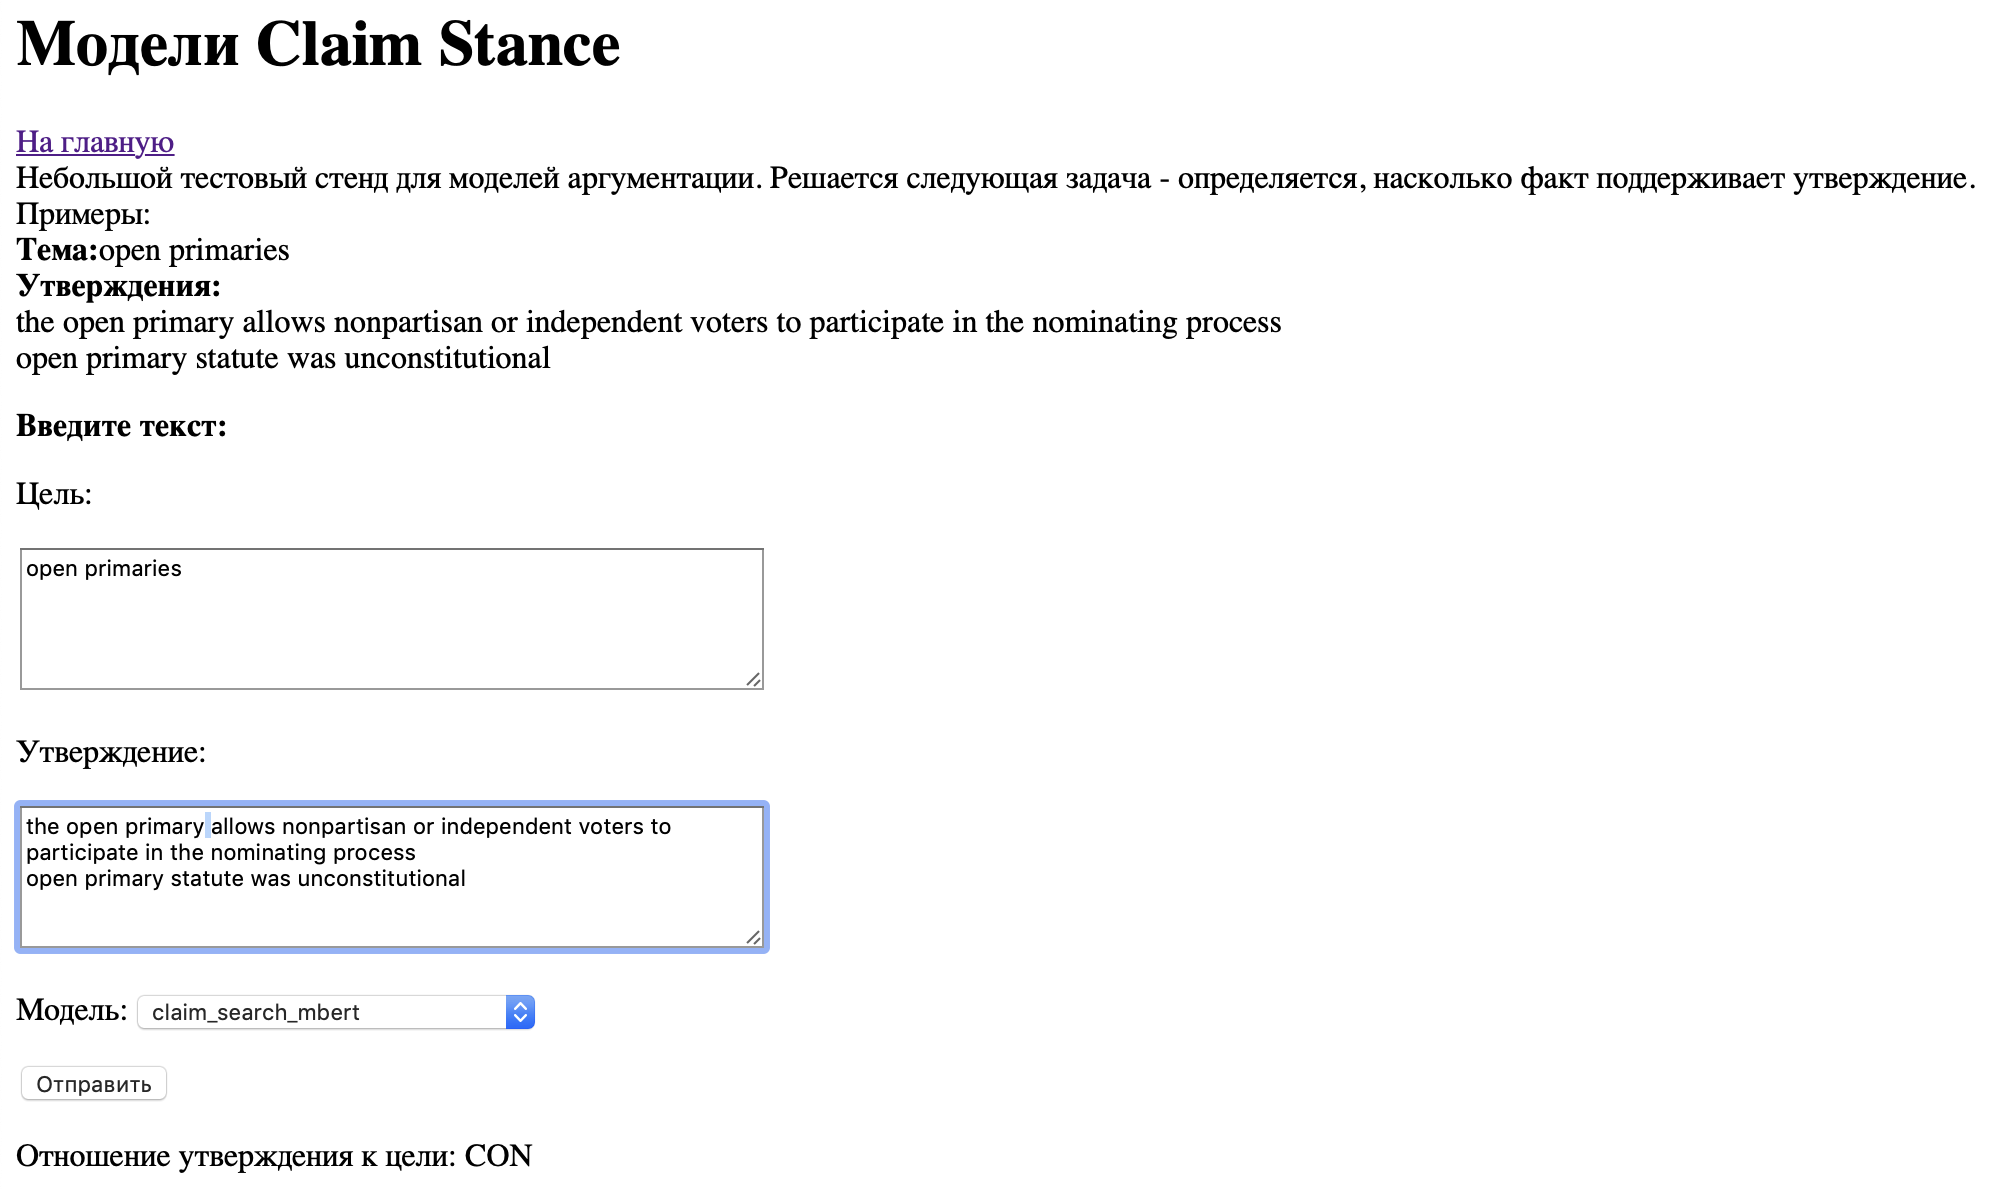
\includegraphics[scale=0.5]{service.png}}
 \caption{Интерфейс сервиса.}
\end{figure}



\begin{comment}
\section{Описание практической части}
\subsection{Экспериментальное исследование}

\subsubsection{Выделение предпосылок}

Первый корпус был взят из работы \cite{aharoni2014benchmark}. Данный корпус состоит из размеченных тем и предпосылок. Всего в корпусе представлено 83 темы. В данном корпусе пары размечены бинарным отношением  наличия релевантности, при этом под релевантностью подразумевается исключительно поддержка, т.е. в рамках данной постановки задачи предпосылки, противоречащие утверждению, имеют тот же класс, что и предпосылки, не имеющие никакого отношения к утверждению. Пример утверждения, относящегося к теме:
\begin{verbatim}
Утверждение: We should increase gun control
Обоснование: Gun control laws are depicted as benign and 
historically progressive.
\end{verbatim}

Для исследования возможности переноса знаний между языками данный корпус был переведен на русский язык.

Так как идейно в этой задаче моделируется связь между двумя высказываниями было решено адаптировать корпуса из задачи Textual Entailment (Natural Language Inference). Был адаптирован русскоязычный корпус TERRa, состоящий из гипотез и предпосылок, которые очень близки к предыдущему корпусу. Пример связанной гипотези и предпосылки:
\begin{verbatim}
Предпосылка: Автор поста написал в комментарии, 
что прорвалась канализация.
Гипотеза: Автор поста написал про канализацию.
\end{verbatim}


Было проведено несколько различных экспериментов. Исследовалась переносимость знаний на русский язык и влияние стороннего корпуса на эффективность переноса знаний. Обучение и валидация происходили на англоязычной версии корпуса. Были обучены следующие вариации моделей:
\begin{itemize}
    \item combined\_mbert\_frozen - мультиязычная модель, обученная на корпусе TERRa и корпусе IBM Evidence Search.
    \item ibm\_mbert\_frozen - мультиязычная модель, обученная на корпусе IBM Evidence Search.
    \item terra\_mbert\_frozen - мультиязычная модель, обученная на корпусе TERRa.
\end{itemize}

Как видно из графиков обучения, лучше всего работает модель ibm\_mbert\_frozen. Как и все названные модели она базируется на модели multilingual BERT. При обучении для применения техники crosslingual transfer у модели замораживается матрица эмбеддингов.

На англоязычной тестовой выборке модели показывают F1-меру около 0.75. При переходе на переведенную русскоязычную версию корпуса качество падает до 0.72-0.73, что говорит об успешном переносе знаний.

\begin{figure}[h!]
  \centering
  \begin{minipage}[b]{0.45\textwidth}
    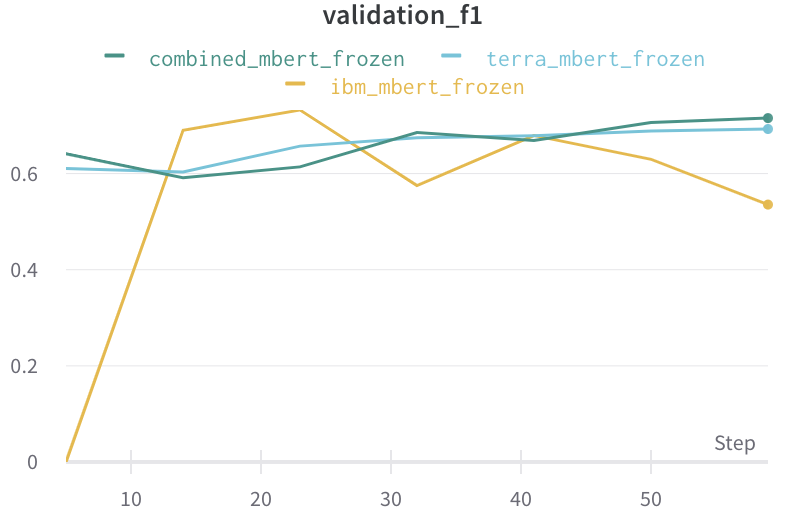
\includegraphics[width=\textwidth]{f1.png}
    \caption{F1-мера на задаче поиска предпосылок.}
  \end{minipage}
  \hfill
  \begin{minipage}[b]{0.45\textwidth}
    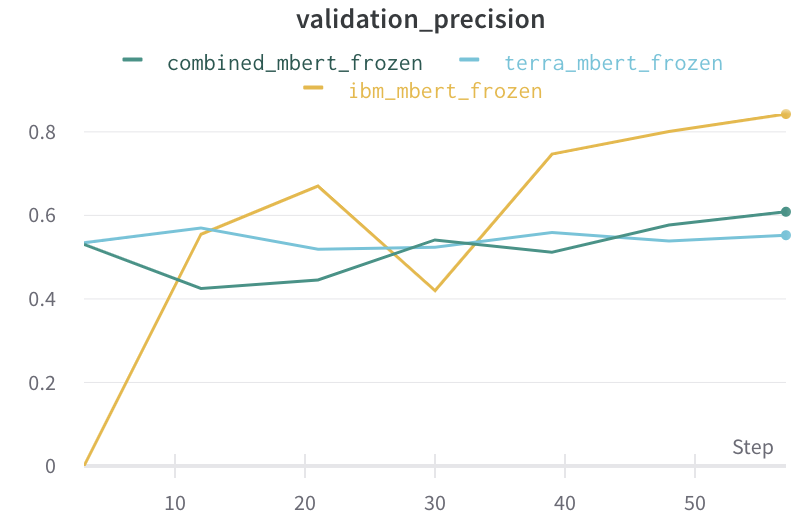
\includegraphics[width=\textwidth]{precision.png}
    \caption{Точность на задаче поиска предпосылок.}
  \end{minipage}
  \begin{minipage}[b]{0.45\textwidth}
    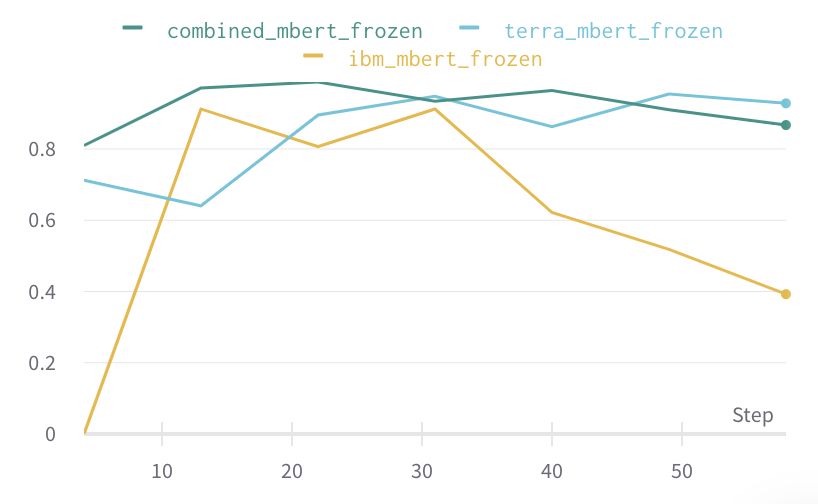
\includegraphics[width=\textwidth]{recall.png}
    \caption{Полнота на задаче поиска предпосылок}
    \label{pd_3}
  \end{minipage}
\end{figure}



Стоит отметить, что на этом корпусе нет установленной таблицы лидеров, поэтому заявленные числа тяжело оценить из-за отсутствия каких-либо конкурентов. Однако ранее упомянутая система MARGOT заявляет об F1-мере в 0.3. Подробные примеры работы можно увидеть в приложении.


\subsubsection{Классификация предпосылок}
У предыдущей постановки задачи существуствует один важный недостаток - она не позволяет различить нейтральную связь от атакующей. Для этого был адаптирован корпус \cite{bar2017stance}, позволяющий определить полемическую позицию аргументации. Под полемической позицеий в данном контексте понимается тип связи между предпосылкой и утверждением или темой. Позиция бывает трех типов: нейтральная, атакующая (опровергающая, противоречащая) и поддерживающая (согласованная). В данном  корпусе размечены аналогичные пары утверждений и предпосылок в отношения атаки и поддержки. В данном корпусе отсутствуют нейтральные отношения. Для этого были дополнительно обработаны исходные тексты, и все тексты, не размеченные в поддержку или атаку считались нейтральными. Пример:
\begin{verbatim}
Утверждение: Реклама вредна
Предпосылка: Реклама распространяет консьюмеризм и культуру потребительства
Вид связи: Поддержка

Утверждение: Бокс полезен
Предпосылка: Бокс остается 8м самым летальным видом спорта
Вид связи: Атака
\end{verbatim}

Вместо задачи бинарной классификации в отношения атаки и поддержки рассматривается задача регрессии в отрезок $[-1; 1]$, где -1 - атака, 1 - поддержка, 0 - нейтральное отношение. Для получения классов данный отрезок был поделен на 3 равные части. По этим частям вышла точность в 62\%.

\begin{figure}[H]
 \captionsetup{justification=raggedright,singlelinecheck=false,labelfont=bf,labelsep=period,name={Рисунок}}
 \centering{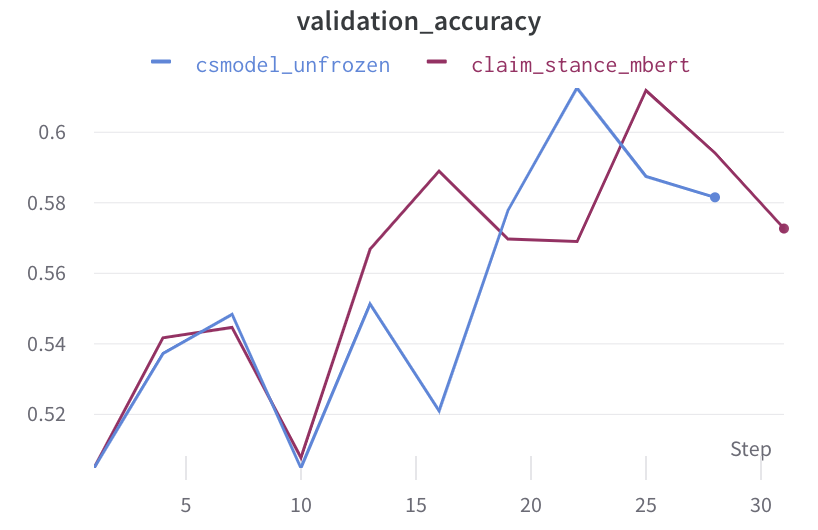
\includegraphics[scale=0.8]{accuracy.png}}
 \caption{Точность системы классификации полемической позиции предпосылок по отношению к утверждениям.}
\end{figure}

Стоит отметить, что в задачах очень сильные сдвиги в распределениях - нейтральных примеров много больше, чем положительных или отрицательных.

\subsubsection{Исследование полученного решения}

С помощью веб-интерфейса проводилось исследование полученных систем. В первую очередь хотелось понять, насколько в модели используется некое внутреннее знание, и насколько в модель опирается на структурные особенности аргумента, такие как общие слова и окрашенную лексику.

Эксперименты показали, что модели улавливает антонимию и отрицания с помощью частицы ``не'', но у модели возникают проблемы со сложными темами, не вошедшими в обучающие корпуса. Проблема данных корпусов в том, что они содержат большое число примеров на ограниченном наборе тем, в то время как в рамках предобученной модели предпочтительнее было бы иметь разнообразное число тем.

\subsection{Обнаружение пропаганды}

Как отмечалось ранее, пропаганда является политической аргументацией, хотя в некоторой литературе ее называют ``ложной'' аргументацией. Было принято участие в соревновании  SemEval 2020 Task 11 Propaganda Detection In News Articles\cite{da2020semeval}. Было представлена два трека - детекция пропаганды и классификация пропаганды. По результатам\cite{dimov-etal-2020-nopropaganda} участия было занято 7 место из 36 в первом треке и 6 из 31 во втором треке.

Корпус состоял из ручной разметки новостных статей за 2019 год. Всего было обработано 438 статей, содержащих 21230 предложений, из которых 7485 содержали пропаганду.

\subsubsection{Определение участков текста с пропагандой}
В первом треке требовалось определить участки текста, являющиеся пропагандой, т.е. постановка задачи заключается в бинарной разметке текста на предмет наличия приемов убеждения. 

\begin{figure}[H]
 \captionsetup{justification=raggedright,singlelinecheck=false,labelfont=bf,labelsep=period,name={Рисунок}}
 \centering{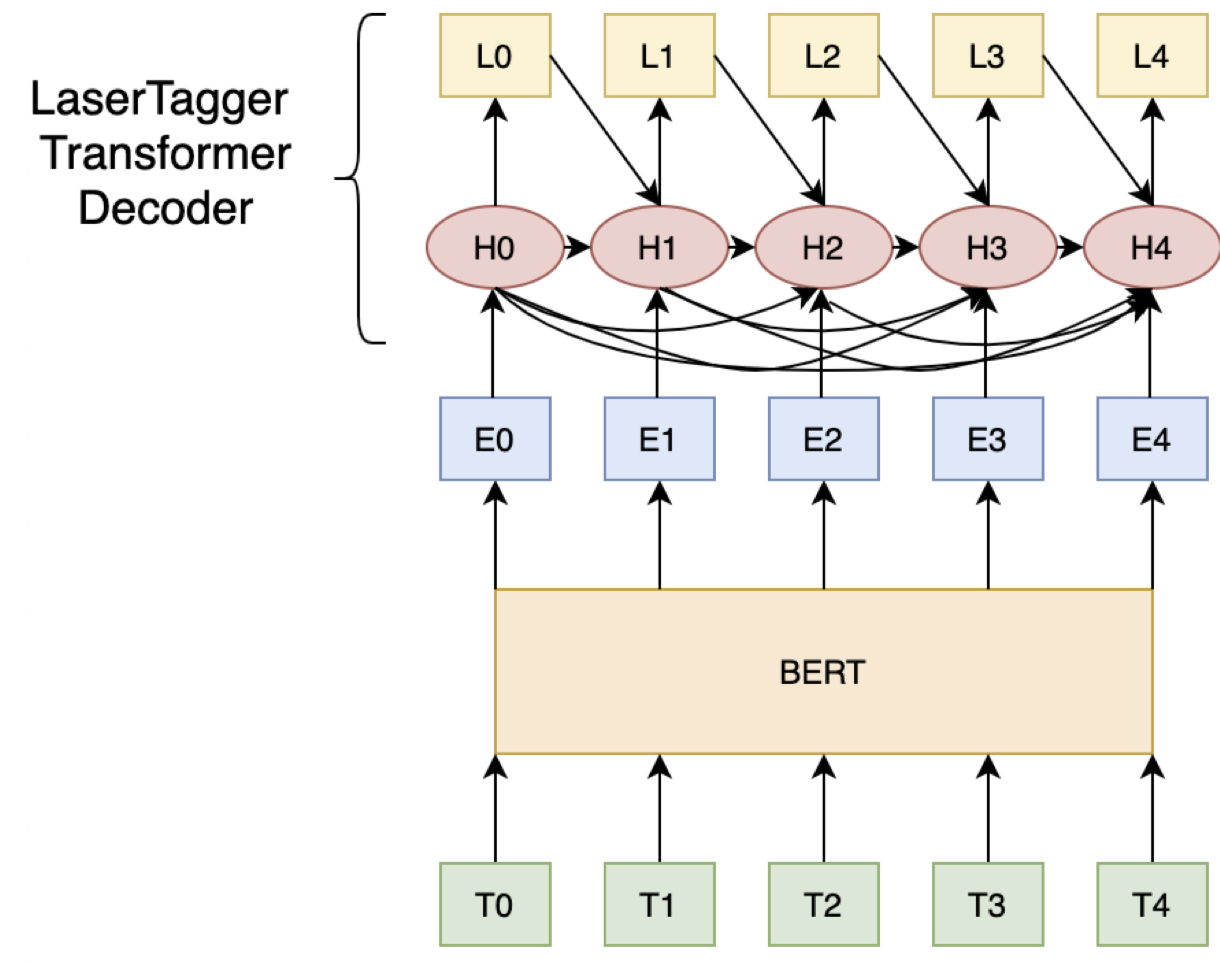
\includegraphics[scale=0.5]{lasertagger.png}}
 \caption{Архитектура LaserTagger из первого трека. $T_i$ - входная последовательность токенов, $L_i$ - бинарные метки для токенов.}
\end{figure}

Т.к. задача тэгирования последовательности, частным видом которой является распознавание именованных суностей, имеет ряд стандартных архитектур, было решено применить несколько стандартных подходов для получения хорошего базового решения.

\begin{figure}[H]
\setcounter{figure}{0}
 \captionsetup{justification=raggedright,singlelinecheck=false,labelfont=bf,labelsep=period,name={Таблица}}
 \centering{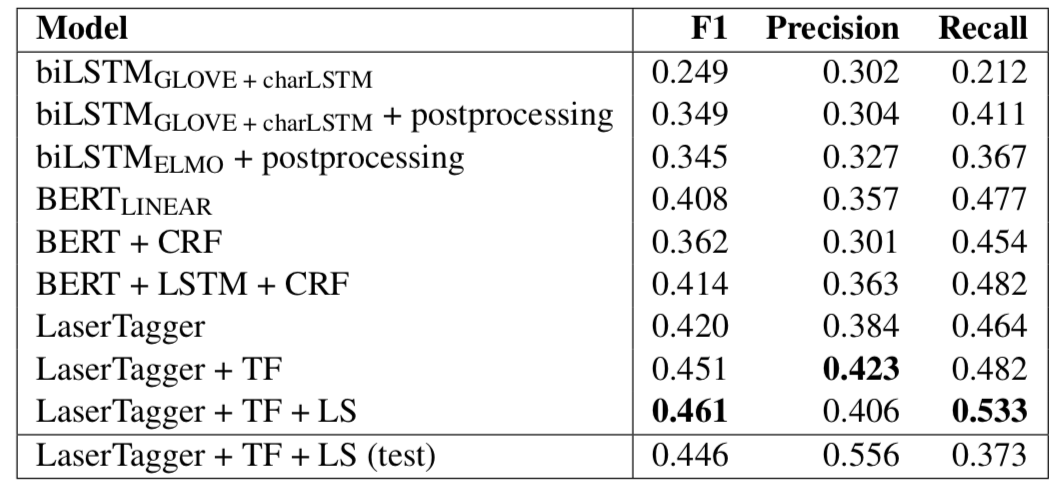
\includegraphics[scale=0.7]{laser_table.png}}
 \caption{Архитектура LaserTagger из первого трека. $T_i$ - входная последовательность токенов, $L_i$ - бинарные метки для токенов.}
\end{figure}

В результате была принята авторегрессионная модель LaserTagger \cite{malmi2019encode}. По сравнению с обычными моделями тэгирования у нее есть одно важное преимущество: она учитывает свои предыдущие предсказания, поэтому она имеет возможность предсказывать длинные непрервыные участки текста без разрывов.

Как видно из таблицы стандартные пододы получают низкие метрики в районе 24-35\% F1-меры. Использование CRF для связного предсказания меток не приносит пользы. Базовая модель, основанная на BERT сразу получает метрику в 40\%.

Для обучения финальной версии архитектуры lasertagger использовалась методика labelsmoothing для смягчения ошибок по краям пропаганды, а также teacher forcing. Teacher forcing заключается в смешивании результатов авторегресионной модели с ее предсказаниями во время обучения. Таким образом получается, что модель ошибается во время обучения и ислледуюет больше пространства и становится более устойчивой к ошибкам.

\subsubsection{Классификация пропаганды}

\cite{wu2019enriching}
Данный трек заключался в классификации участков с пропагандой в один из 18 классов:
\begin{itemize}
    \item Сильно окрашенная лексика. Пример: ".. a lone lawmaker’s childish shouting."
    \item Навешивание ярлыков и имен. Пример: "Republican congressweasels"
    \item Повторение. Заключается в повторении тезиса для закреплении концепции в голове у слушателей.
    \item Преувеличение или приуменьшение. Пример: "Democrats bolted as soon as Trump’s speech ended in an apparent effort to signal they can’t even stomach being in the same room as the president"
    \item Сомнения. Пример: "Is he ready to be the Mayor?"
    \item Взывание к страхам и предрассудкам. Пример: "stop those refugees; they are terrorists"
    \item Сбор под флагом, т.е. взывание к аудитории на почве общей какой-либо общей идентичности (национальности, пола и т.п.). Пример: "entering this war will make us have a better future in our country"
    \item Упрощение причины, т.е. упор на какую-либо первопричину в проблеме с множеством факторов. Пример: "If France had not declared war on Germany, World War II would have never happened."
    \item Слоганы - любые яркие фразы, взывающие к эмоциям. Пример: "Make America great again!"
    \item Диктатура - представление ограниченного выбора в задаче, где существует большее число вариантов решение проблемы. Пример: "There is no alternative to war."
    \item Терминирующие размышления клише - фразы дискредитирующие критичекское размышление по теме обсуждения. Пример: "никто не идеален" или "нельзя изменить человеческую натуру"
    \item Whataboutism - перевод темы для занятия более высокой моральной позиции. Пример: "А у вас права ущемляют!".
    \item Сведение вопроса к заведомо осуждаемой теме. Пример: "Only one kind of person can think this way: a communist!"
    \item Красная сельдь - представление нерелевантной информации для отвращения внимания. 
    \item Стадность - захват мнения через представление позиции, как поддерживаемой большинством. Пример: "Would you vote for Clinton as president? 57\% say yes."
    \item Нарочитая расплывчатость и неясность.
    \item Соломенный человек - подстановка похожего утверждения вместо утверждения оппонента с его последующим опровержением.
\end{itemize}
Классы довольно несбалансированны, поэтому вместо 18 классов для работы модели их число сократили до 14, объединив последние классы в 2 группы. Также стоит отметить, что каждый участок пропаганды может принадлежать более чем одному классу.

\begin{figure}[H]
\setcounter{figure}{12}
 \captionsetup{justification=raggedright,singlelinecheck=false,labelfont=bf,labelsep=period,name={Рисунок}}
 \centering{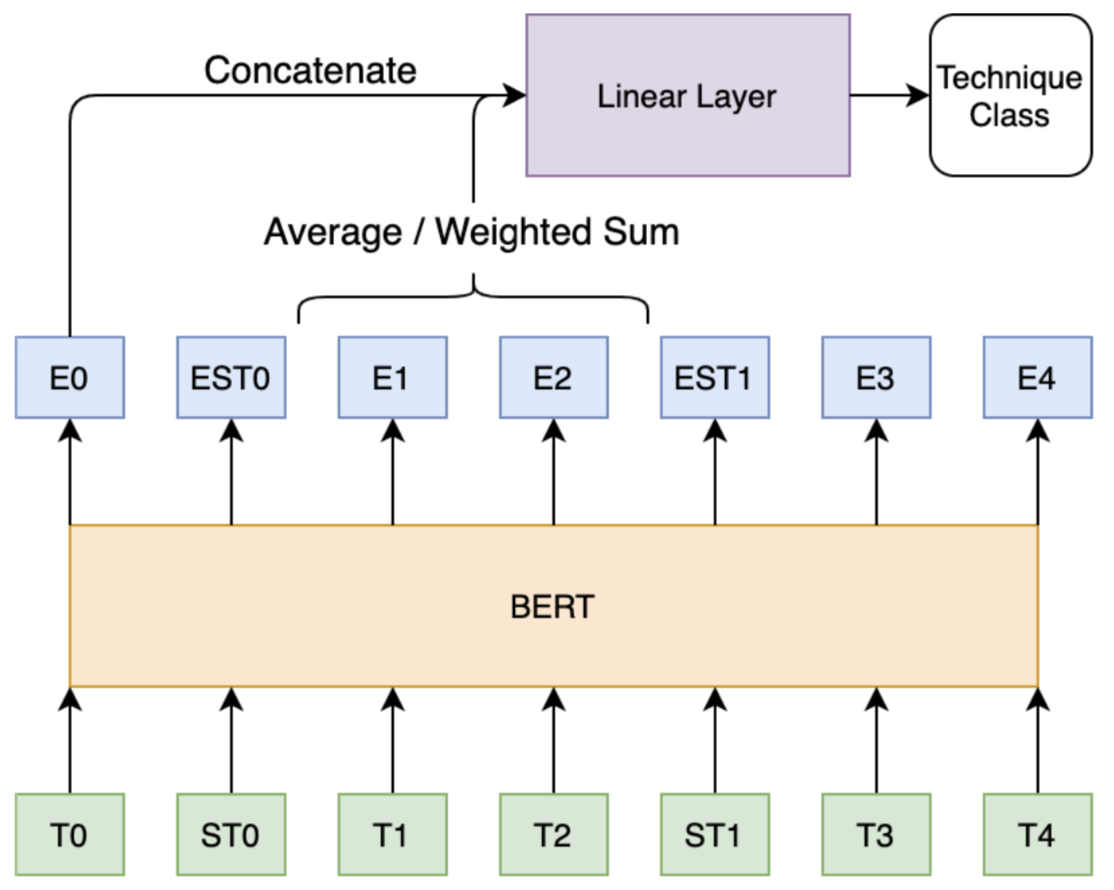
\includegraphics[scale=0.5]{rbert.png}}
 \caption{Результаты моделей классификации пропаганды.}
\end{figure}

Была применена модель RBERT, позаимствованная из задачи извлечения отношений. Особенностью данной модели является обособление участков текста спецсимволами. Также было использовано несколько обычных моделей классификации.

В модели RBERT был использован механизм пулинга через веса, полученные в результате работы механизма внимания.В конечной посылке был использован ансамбль обученных моделей.

\begin{figure}[H]
\setcounter{figure}{1}
 \captionsetup{justification=raggedright,singlelinecheck=false,labelfont=bf,labelsep=period,name={Таблица}}
 \centering{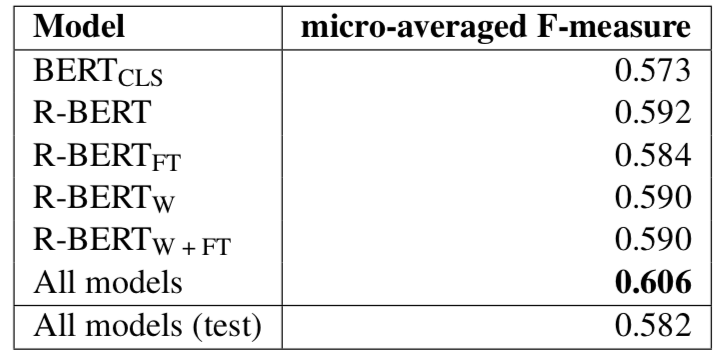
\includegraphics[scale=0.7]{rbert_table.png}}
 \caption{Архитектура RBERT из второго трека. $T_i$ - входная последовательность токенов, $E_i$ - внутреннее представление токенов в модели.}
\end{figure}


\subsubsection{Исследование полученного решения}
Анализ ошибок модели выделения пропаганды показал, что данная модель имеет и некоторые недостатки: модель часто выделяет различные обособленные обороты и цитаты полностью, вместо их частей. Выделение цитат легко объяснить - они очень часто содержат речь, которая более эмоционально и содержит самый частый класс пропаганды. Также модель иногда наоборот закрывает участок с пропагандой при переходе через запятую и не открывает участок заново.

Часть проблем возникает и из-за особенностей корпуса. В корпусе прослеживается сильное смещение тем между тестовой выборкой и тренировочной, валидационной. Из-за этого метрики всех участников на валидационной выборке на 10-15\% выше, чем итоговые результаты на тесте.

Анализ модели классификации выявил, что она хорошо выделяет частотные классы, но хуже справляется с редкими.

Две команды, занявшие первые места в треках, использовали более простые  модели для тэгирования последовательности, однако обе использовали подход активной доразметки других открытых корпусов, что говорит о том, что и предложенные в этой работе системы могут быть улучшены за счет увеличения обучающей выборки.

\subsection{Программная реализация}
Код\footnote{https://github.com/hawkeoni/Thesis.}, сопровождающий данную работу, написан на языке Python 3.6.x и логически разделяется на следующие компоненты с соответствующими объемами:
\begin{itemize}
    \item Логика веб-приложения - обработка запросов и применение моделей. 80 строк кода на языке Python.
    \item Страницы веб-приложения - 100 строк на HTML.
    \item Javascript сценарии для удобного интерфейса веб-приложения - 60 строк.
    \item Код для предобработки данных в формат удобный для обучения из таких форматов как CSV, JSON, XML, MySQL dump - 720 строк.
    \item Код для обучения - нейросетевый модели, преобразование данных в многомерные массивы, логирование метрик, составляет 335 строк.
    \item Код для доступа к онлайн интерфейсам для перевода текстов - 81 строка.
    \item Конфигурационные JSON-файлы для архитектуры моделей и стратегии их обучения - 370 строк.
\end{itemize}

Ради скорости прототипирования для разработки приложения был выбран микро-фреймворк Flask версии 1.1.1. Для написания и обучения нейросетевых архитектур используется связка библиотеки Pytorch\cite{pytorch} версии 1.6.0 и AlleNLP\cite{allennlp} версии 1.1.0. Совокупность данных библиотек позволяет удобным образом писать конфигурации для экспериментов в формате JSONNET. Пример подобного конфигурационного файла можно посмотреть в \hyperref[sec:jsonnet]{приложении}. Большие предобученные языковые модели, такие как \textbf{BERT, ROBERTa, ruBERT} и т.п. были взяты из библиотеки Transformers\cite{transformers} версии 3.0.2.

Прогресс обучения моделей логируется в онлайн-сервисе wandb\footnote{https://wandb.ai/hawkeoni}.

\begin{figure}[H]
\setcounter{figure}{13}
 \captionsetup{justification=raggedright,singlelinecheck=false,labelfont=bf,labelsep=period,name={Рисунок}}
 \centering{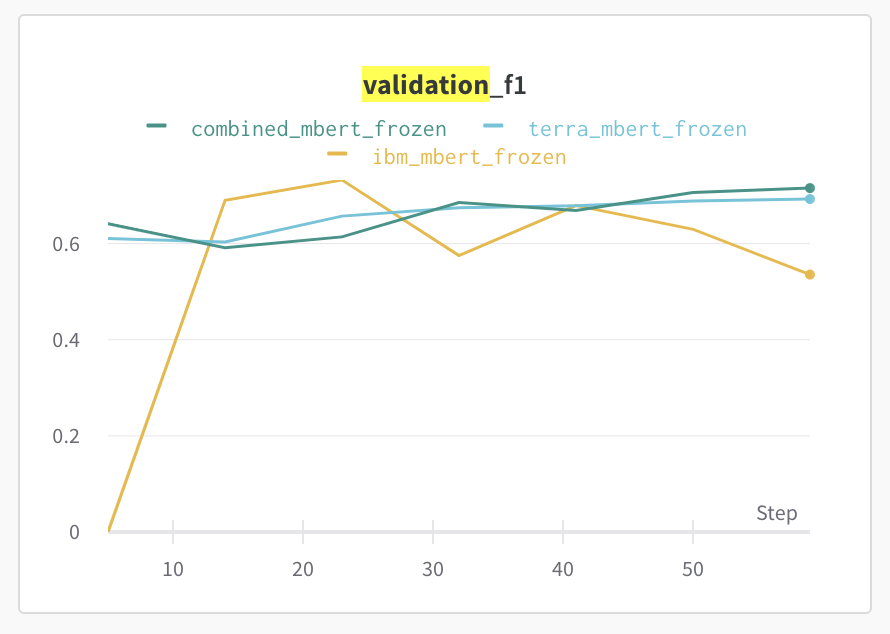
\includegraphics[scale=0.8]{wandb.png}}
 \caption{Пример графика, логируемого в сервис wandb.}
\end{figure}

Дополнительно для удобства веб-приложение собрано в Docker-контейнер.

\subsection{Описание веб-сервиса}
\begin{figure}[H]
 \captionsetup{justification=raggedright,singlelinecheck=false,labelfont=bf,labelsep=period,name={Рисунок}}
 \centering{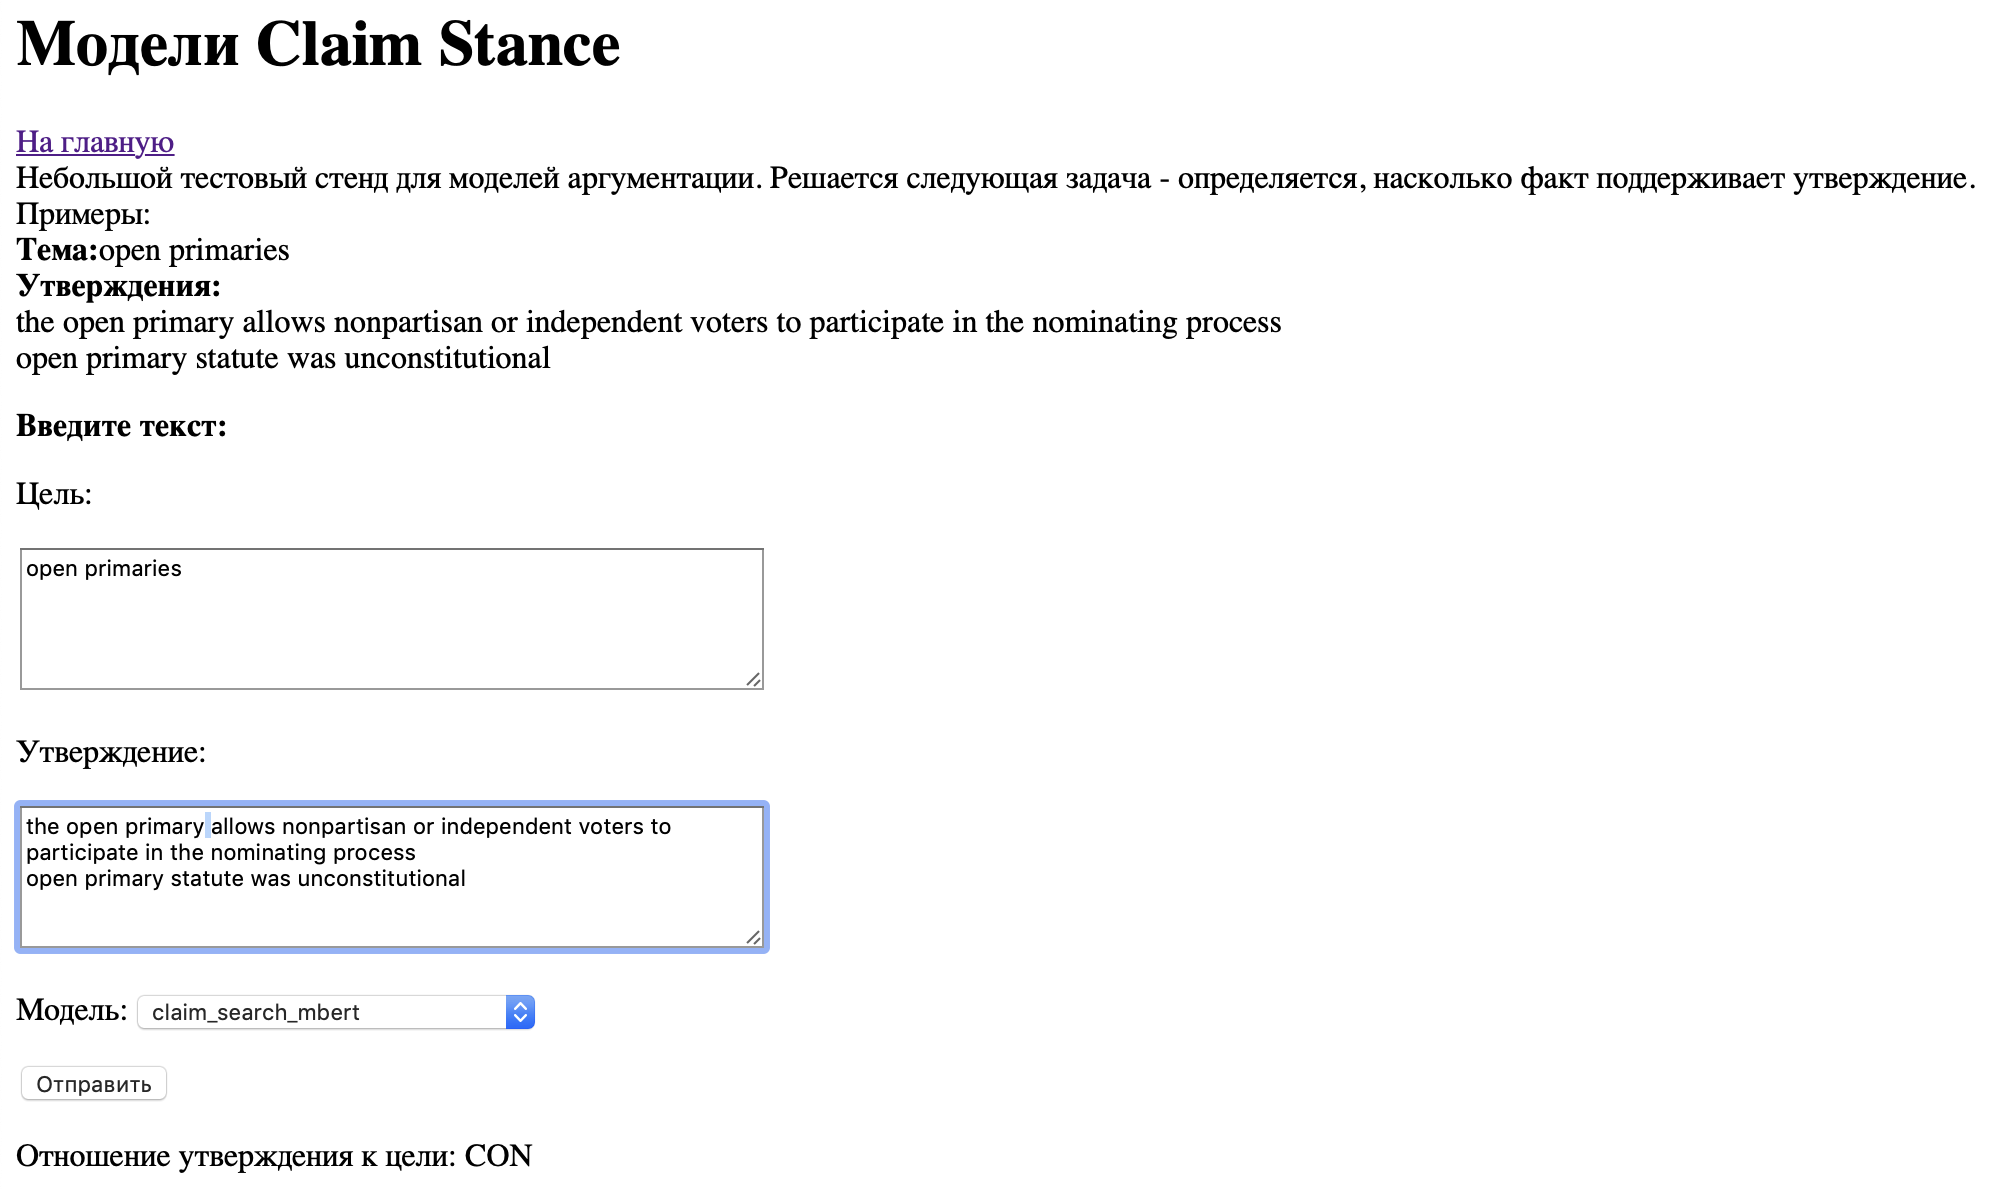
\includegraphics[scale=0.5]{service.png}}
 \caption{Интерфейс сервиса.}
\end{figure}
Для исследования эффективности работы моделей извлечения аргументации было создано веб-приложение. Веб-приложение содержит в себе 3 страницы, 2 из которых позволяют взаимодействовать с моделями.

Первая страница посвещена определению предпосылки по утверждению, а вторая страница классифицирует отношение между утверждением и предпосылкой. Каждая страница имеет 3 поля:
\begin{itemize}
    \item Поле для утверждения или темы.
    \item Поле для предпосылки.
    \item Поле для выбора моделей.
\end{itemize}

Отображение реализовано через JavaScript, поэтому результат работы модели получается без перехода на новую страницу. Для удобства анализа модели возвращается не только полученный класс связи, но также внутреннее представление модели - ее уверенность в полученном ответе.
\end{comment}
\section{Экспериментальное исследование}

\subsection{Эксперименты на корпусе IBM Evidence Search}

Для первых экспериментов для извлечения структуры аргументации был выбран корпус IBM Evidence Search из работы \cite{shnarch2018will}. В рамках данной текстовой коллекции необходимо найти связь между темой и предпосылкой. Примеры:

\begin{verbatim}
    Тема: We should fight illegal immigration
    Предпосылка: A paper in the peer reviewed Tax Lawyer journal from the American 
    Bar Association asserts that illegal immigrants contribute more in taxes 
    than they cost in social services
    Тип отношения: релевантно
    
    Тема: We should abandon coal mining
    Предпосылка: In particular, Daintree was the first Government geologist for
    North Queensland discovering gold fields and coal seams for future exploitation.
    Тип отношения: нерелевантно
\end{verbatim}

В данном корпусе представлено 5700 пар тем и предпосылок по 118 темам, 35 из которых отведены в качестве тестовой выборки. Примеров положительного класса, т.е. пар релевантных темы и посылки и в тестовой и в обучающей части около 40\%. Дополнительно тестовая часть этого корпуса была переведена на русский язык для замеров эффективности межязыкового переноса.

Также рассматривается русскоязычный корпуса TERRa. В данном корпусе стоит задача логического вывода: необходимо по паре текста и гипотезы понять, можно ли вывести гипотезу из текста. Данная постановка похожа на постановку определения релевантности, поэтому было решено исследовать влияние обучения на корпусе TERRa на решение задачи определения структуры аргументации. Пример данных из корпуса TERRa:
\begin{verbatim}
    Текст: Женщину доставили в больницу, за ее жизнь сейчас борются врачи.
    Гипотеза: Женщину спасают врачи.
    Тип отношения: гипотезу можно вывести из текста
    
    Текст: Представитель внешнеполитического ведомства отметил, что злоумышленника
    задержали местные власти.
    Гипотеза: Злоумышленник напуган.
    Тип отношения: гипотеза не следует из текста.
\end{verbatim}

\begin{table}[h!]
\centering
\begin{tabular}{|| c | c | c |} 
 \hline
 Модель & Макро-Точность & Микро-Точность \\ [0.5ex] 
 \hline
 $BERT_{en}$ & \textbf{82.4} & \textbf{81.1} \\ 
 $BERT_{mult}$ & 81.6 & 80.5 \\
 $IBM BiLSTM$ & - & 72 \\
 $IBM BiLSTM_{ext}$ & - & 76 \\ 
 \hline
 $BERT_{mult}$ & 77.5 & 76.4 \\
 $BERT_{terraZS}$ & 66.7 & 60.3 \\
 $BERT_{comb}$ & 75.9 & 73.9 \\
 \hline
\end{tabular}
\caption{Результаты на тестовом корпусе IBM Evidence Search. Горизонтальной линией отделены результаты на англоязычной и русскоязычной версиях.}
\label{table:1}
\end{table}

В качестве метрики в исходной работе используется микро-точность по темам. В качестве моделей авторы \cite{shnarch2018will} предлагали двунаправленную LSTM над векторизацией слов GloVE. Данная модель обозначена как $IBM BiLSTM$. Авторы также исследовали влияние внешних данных, собранных автоматически на качество работы модели. Модель, использующая внешние данные называется $IBM BiLSTM_{ext}$. Автоматически собранный корпус не выложен в открытый доступ, поэтому исследовать его влияние на предложенные в данной дипломной работе модели не представляется возможным.

В качестве предложенных моделей для обучения на английском корпусе было решено взять архитектуру $BERT_{base}$, т.е. модель, одновременно обрабатывающую обе компоненты аргументации. В таблице 1 моделью $BERT_{en}$ называется модель на архитектуре $BERT_{base}$, дообученная с весов англоязычной версии $BERT$. Модели $BERT_{mult}$, $BERT_{terraZS}$, $BERT_{comb}$ дообучены с весов мультиязычной версии оригинальной модели $BERT$.

Как видно из таблицы использование англоязычной модели $BERT_{en}$ дает заметно лучшее качество, чем модели, основанные на архитектуре $BiLSTM$, даже с использованием внешних данных. На один пункт точности уменьшается качество мультиязычной модели $BERT_{mult}$ по сравнению с англоязычной, но качество все еще заметно выское.

Во второй половине таблицы отображены результаты работы модели $BERT_{mult}$ на русскоязычной версии корпуса. Происходит заметное падение качества на 5 пунктов, однако модель все еще извлекает аргументацию на уровне, сопоставимом с наилучшим решением.

Модель $BERT_{terraZS}$ была обучена на корпусе TERRa и применена в сценарии Zero Shot (без дообучения) на корпусе IBM Evidence Search. Модель показывает ненулевое качество. Дальнейшей попыткой применить корпус логического вывода TERRa является модель $BERT_{comb}$. Было решено объединить корпуса TERRa и IBM Evidence Search, чтобы понять как влияет корпус TERRa на задачу извлечения структуры аргументации. Полученная модель оказывается хуже аналогичной модели $BERT_{mult}$, обученной исключительно на англоязычных данных.

\subsection{Эксперименты на корпусах ArgsEN и EviEN}
В новой работе \cite{toledo2020multilingual} предоставлено 2 корпуса, посвященных аргументации: ArgsEN и EviEN. В корпусе ArgsEN на 30000 примеров размечена полемическая позиция между темами и утверждениями:

\begin{verbatim}
    Тема: We should abandon marriage
    Утверждение: \"marriage\" isn't keeping up with the times.  abandon the old
    thinking and bring something that incorporates all unions - not just those with a
    man and woman.
    Полемическая позиция: поддержка
    
    Тема: We should prohibit flag burning
    Утверждение: a flag is only really a peace of cloth and doesn't actually hurt
    anybody.
    Полемическая позиция: противоречие (атака)
\end{verbatim}

В корпусе EviEN похожим образом размечены отношения между темами и предпосылками (35000 пар), дополнительно размечена и релевантность. Таким образом корпус EviEN является единственным корпусом, на котором можно решать одновременно задачи извлечения струкутуры и определения полемической позиции. Примеры:

\begin{verbatim}
    Тема: We should ban the sale of violent video games to minors
    Предпосылка: Justice Thomas, in his dissent, considered that historically, 
    the Founding Fathers "believed parents to have complete authority over 
    their minor children and expected parents to direct the 
    development of those children
    Структура: релевантно
    Полемическая позиция: противоречие
    
    Тема: We should ban the sale of violent video games to minors
    Предпосылка: while owning guns is a legal right in most countries, 
    the illegal trade in guns continues to fuel conflict
    Структура: нерелевантно
    Полемическая позиция: нейтральная
\end{verbatim}

Также дополнительно рассматриваится и корпус для логического вывода SNLI. Данный корпус состоит из 570000 пар текстов и гипотез, необходимо определить поддерживается, опровергается гипотеза текстом или из текста нельзя сделать выводы о гипотезе. Примеры:

\begin{verbatim}
    Тема: A person on a horse jumps over a broken down airplane.
    Гипотеза: A person is outdoors, on a horse.
    Отношение: Подтверждение
\end{verbatim}

На корпусе ArgsEN проводились замеры качества определения полемической позиции аргументации, отображенные в таблице 2.


\begin{table}[h!]
\centering
\begin{tabular}{|| c | c |} 
 \hline
 Модель & Макро-F1 \\ [0.5ex] 
 \hline
 $IBM BERT_{en}$ & 89.3 \\
 $IBM BERT_{17L}$ & \textit{91.5} \\
 $BERT_{basic}$ & 90.1 \\
 $BERT_{vectorized}$ & 75.2 \\
 $BERT_{SE}$ & \textbf{90.3} \\
 $BERT_{snliZS}$ & 55.0 \\
 $BERT_{snliFT}$ & 87.9 \\
 \hline
\end{tabular}
\caption{Результаты на тестовом корпусе ArgsEN в задаче определения полемической позиции утверждения относительно темы. Метрика - макроусредненная F1 по темам.}
\label{table:1}
\end{table}

Авторы оригинальной работы представляют результаты моделей $IBM BERT_{en}$ и $IBM BERT_{17L}$. Архитектуры моделей не описываются, известно, что первая модель училась на английском корпусе, а вторая модель училась на неопубликованном корпусе из 17 языков. Вторая модель показывает наилучшие результаты и включена в сравнение для предоставление как лучшая обученная модель, однако предоставленные в данной дипломной работе модели справедливо сравнивать лишь с первой моделью, т.к. они учились исключительно на английском языке. 

Модели $BERT_{basic}$, $BERT_{vectorized}$, $BERT_{SE}$ начинали обучение с англоязычных весов модели $BERT$ и представляют собой архитектуры, описанные в 4 главе. Модель $BERT_{vectorized}$ из-за отсутствия перекрестного механизма внимания, вызванного независимой обработкой компонент аргументации показывает низкий результат. Значительно лучше ведет себя модель $BERT_{basic}$, способная смоделировать сложные завивимости между темой и утверждением, так как они подаются в модель одновременно. Модель со слоем интерпретации $BERT_{SE}$ показывает результат немного превосходящий базовую модель.

Дополнительно использовалась модель обученная на корпусе SNLI. В оригинальном корпусе SNLI присутствует 3 отношения: поддержка, атака и нейтральное отношение. Т.к. в данном корпусе нет нерелевантных пар темы и утверждения, из предсказаний модели выбирается наиболее вероятный класс из поддержки или атаки. В сценарии без дообучения (Zero Shot) модель $BERT_{snliZS}$ показывает низкий результат в 55 пунктов точности на задаче бинарной классификации. Дообученная модель $BERT_{snliFT}$ показывает также показывает более низкий результат, чем модель $BERT_{basic}$. Данный результат совпадает со схожим экспериментом на корпусах IBM Evidence Search и TERRa.

На корпусе EviEN тоже присутствует возможность выделять полемическую позицию, однако авторы работы \cite{toledo2020multilingual} не предоставляют для сравнения никаких модельных результатов. Модели, аналогичные моделям для корпуса ArgsEN представлены в таблице 3.

\begin{table}[h!]
\centering
\begin{tabular}{|| c | c |} 
 \hline
 Модель & Макро-F1 \\ [0.5ex] 
 \hline
 $BERT_{basic}$ & 64.8 \\
 $BERT_{vectorized}$ & 51.8 \\
 $BERT_{SE}$ & 67.6 \\
 \hline
\end{tabular}
\caption{Результаты на тестовом корпусе EviEN в задаче определения структуры и полемической позиции предпосылки относительно темы. Метрика - макроусредненная F1 по темам.}
\label{table:1}
\end{table}



Как отмечалось ранее, на корпусе EviEN поставлена вторая задача определения релевантности предпосылки по отношению к теме. Авторы корпуса не предоставляют своих модельных метрик. Метрики моделей из главы 4 предоставлены в таблице 4:

\begin{table}[h!]
\centering
\begin{tabular}{|| c | c |} 
 \hline
 Модель & Макро-F1 \\ [0.5ex] 
 \hline
 $BERT_{basic}$ & 68.5 \\
 $BERT_{vectorized}$ & 64.3 \\
 $BERT_{SE}$ & 72.8 \\
 \hline
\end{tabular}
\caption{Результаты на тестовом корпусе EviEN в задаче определения структуры аргументации (релевантности). Метрика - макроусредненная F1 по темам.}
\label{table:1}
\end{table}

Результаты на корпусе ArgsEN превосходят модели, предложенные в работе \cite{toledo2020multilingual} по метрикам. На всех корпусах лучше всего себя показывает модель $BERT_{SE}$ со слоем интерпретации, а хуже всего модель $BERT_{vectorized}$.


\subsection{Обнаружение пропаганды}
Корпус пропаганды состоял из ручной разметки новостных статей за 2019 год. Всего было обработано 438 статей, содержащих 21230 предложений, из которых 7485 содержали пропаганду.

В качестве первого трека были даны новостные статьи и было необходимо выделить участки текста, содержащие пропаганду.

\begin{table}[h!]
\centering
\begin{tabular}{|| c | c | c | c |} 
 \hline
 Модель & F1 & Precision & Recall \\ [0.5ex] 
 \hline
 $BiLSTM_{glove+charlstm}$ & 34.9 & 30.4 & 41.1 \\
 $BiLSTM_{ELMO}$ & 34.5 & 32.7 & 36.7 \\
 $BERT_{linear}$ & 40.8 & 35.7 & 47.7 \\
 $BERT_{crf}$ & 36.2 & 30.1 & 45.4 \\
 $BERT_{lstm+crf}$ & 41.4 & 36.3 & 48.2 \\
 $LaserTagger$ & 42.0 & 38.4 & 46.4 \\
 $LaserTagger{tf}$ & 45.1 & 42.3 & 48.2 \\
 $LaserTagger{tf+ls}$ & 46.1 & 40.6 & 53.3 \\
 \hline
 $LasterTagger_{TF+LS}$ & 44.6 & 55.6 & 37.3 \\
 $Hitachi$ & 51.5 & 56.5 & 47.3 \\
 \hline
\end{tabular}
\caption{Результаты на задаче выделения пропаганды. В качестве метрики используется посимвольная F1-мера. Чертой отделены замеры на валидационной выборке и тестовой.}
\label{table:1}
\end{table}

В качестве базовых моделей были предложены архитектуры на основе рекуррентной нейросети BiLSTM. Модель $BiLSTM_{glove+charlstm}$ использует для векторизации эмбеддинги GloVe и буквенный рекуррентный слой BiLSTM. Данный подход позволяет обрабатывать слова, которые не встречались в исходном словаре GloVe. Второй вариацией данной модели является векторизация на основе буквенной нейросети ElMO \cite{Peters:2018}. Из таблицы 5 видно, что два этих подхожа не имеют большой качественной разницы.

Далее ведется работа с англоязычной версией нейросетевой модели $BERT$. Модель, в которой слова векторизуются $BERT$ и подаются в линейный слой называется $BERT_{linear}$, что дает большой прирост качества относительно базовых моделей. Минусом данной модели является независимое предсказание последовательности меток. Для решения данной проблемы использовалась нейросеть $BERT_{crf}$, в которой слой Conditional Random Field одновременно оценивает всю последовательность меток, однако данный метод не дает улчшения, а наоборот ухудшает результат.

В качестве продолжения идеи научить модель связанно предсказывать метки была принята архитекутра $LaserTagger$. Данная модель работает аналогично моделям машинного перевода - исходная последовательность проходит векторизацию моделью $BERT$, после чего каждому слову в соответстиве ставится метка. В качестве модификаций данной модели были предложены методики Teacher Forcing и Label Smoothing, комбинация которых и вошла в финальную модель с качеством 44.6 посимвольной F1-меры.


\begin{table}[h!]
\centering
\begin{tabular}{|| c | c |} 
 \hline
 Модель & Микро-F1 \\ [0.5ex] 
 \hline
 $BERT_{CLS}$ & 57.3 \\
 $R-BERT$ & 59.2 \\
 $R-BERT_{ft}$ & 58.4 \\
 $R-BERT_{w}$ & 59.0 \\
 $R-BERT_{w+ft}$ & 59.0 \\
 $Ensemble$ & 60.6 \\
 \hline
 $Ensemble$ & 58.2 \\
 $ApplicaAI$ & 62.07 \\
 \hline
\end{tabular}
\caption{Результаты на задаче классификации пропаганды. В качестве метрики используется микро-F1 по классам пропаганды. Чертой отделены замеры на валидационной выборке и тестовой.}
\label{table:1}
\end{table}

Для классификации участков пропаганды была выбрана модель $R-BERT$. Для работы данной модели необходимо обрамить участки с пропагандой спецсимволами, чтобы указать модели, какой участок текста является наиболее важным. В базовом варианте для классификации бралось усреднение контекстных векторных представлений выделенного сегмента. В модели $R-BERT_{w}$ модель выучивала веса для участков текста и брала взвешенную сумму их векторных представлений для классификации. В модели $R-BERT_{ft}$ исходная модель $BERT$ дообучалась на доменном корпусе новостей, что дало небольшой прирост качества. В финальной модели использовался ансамбль всех моделей, собранный в голосующий классификатор.


Стоит отметить, что в корпусе прослеживается сильное смещение тем между тестовой выборкой и тренировочной, валидационной. Из-за этого метрики всех участников на валидационной выборке на 10-15\% выше, чем итоговые результаты на тесте. Команды Hitachi и ApplicaAI применили модели, схожие с $BERT_{linear}$, однако использовали внешние данные и методики доразметки данных моделью для радикального увеличения тренировочной выборки. По результатам\cite{dimov-etal-2020-nopropaganda} участия было занято 7 место из 36 в первом треке и 6 из 31 во втором треке.

\section{Заключение}

В рамках данной работы были получены следующие результаты:
\begin{itemize}
    \item Проведен обзор существующих методов и корпусов для извлечения аргументации.
    \item Обучены системы, основанные на больших предобученных языковых моделях, для извлечения аргументации.
    \item Реализован базовый вариант переноса знаний на русский язык для задачи извлечения структуры аргументации.
    \item Исследована возможность использования предобучения на задаче логического вывода для улучшения результатов на задачах извлечения аргументации.
    \item Реализована система для обнаружения пропаганды в новостных ресурсах.
    \item Реализовано базовое веб-приложение для взаимодействия с моделями.
\end{itemize}

В данной работе исследованы задачи автоматического выявления аргументации на примере извлечения структуры и определении полемической позиции аргументации. Несмотря на отсутствие крупных корпусов, на которых исследовательские группы целеноправленно сравнивали бы свои модели, были выделены избранные коллекции. На коллекциях ArgsEN \cite{toledo2020multilingual} в задаче определения полемической позиции аргументации был улучшен результат англоязычной модели с 89.3 пунктов макро F1-меры до 90.3; на коллекции IBM Evidence Search \cite{shnarch2018will} для определения структуры аргументации также улучшен результат с 76 пунктов микро точности до 81.1. На коллекциях, где отсутствовали авторские замеры были также предоставлены показатели качества: на корпусе EviEN на задаче определения полемической позиции - 67.6, на задаче определения структуры аргумента (релевантности) - 72.8.

На корпусе IBM Evidence Search было проведено исследование возможности использования мультиязычной модели для переноса знаний на русский язык. Для этого тестовая выборка была переведена на русский язык. Модель показывает падение точности с 80.5 пунктов для англоязычного корпуса до 76.4 пунктов, что отражает ожидаемое ухудшение качество при смене языка. Тем не менее качество этой модели достигает современного уровня извлечения аргументации. 

Дополнительно на корпусе IBM Evidence Search была исследована возможность применения закономерностей, выученных моделью на корпусе логического вывода. Использование корпуса TERRa в сценарии без дообучения показывает возможность применения подобного решения на задаче определения структуры аргументации. Обучение одновременно логическому выводу и структуре аргументации приводит к ухудшению качества, полученного исключительно на корпусе аргументации, что говорит о непригодности использования корпуса TERRa в подобном сценарии. Аналогичные испытания проводились и для корпуса ArgsEN на задаче определения полемической позиции и корпусе SNLI для логического вывода. В этом эксперименте дообученная модель также привела к ухудшению качества по сравнению с моделью, использующей исключительно корпус аргументации.

Дополнительно исследована задача извлечения пропаганды - частного вида аргументации. Предоставлены модели, занявшие 6 и 7 место в научном семинаре Semeval 11 \cite{dimov-etal-2020-nopropaganda}.

Для взаимодействия с моделями предоставлен веб-сервис, позволяющий для пар компонент аргументации оценить релевантность и полемическую позицию.

В качестве будущего развития работы можно предложить:
\begin{itemize}
    \item Дополнение моделей внешними знаниями для моделирования более сложных зависимостей.
    \item Использование полученных аргументов для создания карт аргументации или генерации текста.
    \item Создание русскоязычной коллекции для решения задачи извлечения аргументации.
\end{itemize}

\bibliographystyle{gost780u.bst} % Для соответствия требованиям об оформлении списка литературы
\bibliography{refs}

% \appendix
% \section{Приложение}
\subsection{Примеры работы сервиса}
\subsection{Поиск предпосылок}

\begin{verbatim}
Утверждение: Мы должны отменить электронное голосование
Предпосылка:Были высказаны предположения, что электронное голосование 
может быть проще и быстрее, чем физическое прохождение 
через холл подразделения.
Связь: Предпосылка поддержвает утверждение

Утверждение: Мы должны запретить азартные игры
Предпосылка: Вообще говоря, избранные вожди и Воинское общество поддерживали
азартные игры, в то время как традиционные вожди выступали против нее.
Связь: Либо нерелевантно, либо отрицание.
\end{verbatim}

\subsection{Классификация отношений}
\begin{verbatim}
Тема: the sale of violent video games to minors
Предпосылка: exposure to violent video games causes at least a temporary increase 
in aggression and that this exposure correlates with aggression in the real world
Связь: Атака

Тема: make physical education compulsory
Предпосылка: A sedentary lifestyle plays a significant role in obesity
Связь: Поддержка

Тема: freedom of speech
Предпосылка:  nuclear weapons contribute to stability at a strategic level
Связь: нейтральная
\end{verbatim}

\subsection{Пример конфигурационного файла для обучения}
\label{sec:jsonnet}
\begin{verbatim}
{
    "dataset_reader" : {
        "type": "IBMReader"
    },
    "train_data_path": "path/to/train/data",
    "validation_data_path": "path/to/validation/data",
    "model": {
        "type": "topic_sentence_model"
    },
    "data_loader": {
        "batch_size": 16
    },
    "trainer": {
        "optimizer": {
            "type": "adam",
            "lr": 2e-5
        },
        "num_epochs": 5
    }
}
\end{verbatim}

\end{document}